\documentclass{beamer}\usepackage[]{graphicx}\usepackage[]{color}
% maxwidth is the original width if it is less than linewidth
% otherwise use linewidth (to make sure the graphics do not exceed the margin)
\makeatletter
\def\maxwidth{ %
  \ifdim\Gin@nat@width>\linewidth
    \linewidth
  \else
    \Gin@nat@width
  \fi
}
\makeatother

\definecolor{fgcolor}{rgb}{0.345, 0.345, 0.345}
\newcommand{\hlnum}[1]{\textcolor[rgb]{0.686,0.059,0.569}{#1}}%
\newcommand{\hlstr}[1]{\textcolor[rgb]{0.192,0.494,0.8}{#1}}%
\newcommand{\hlcom}[1]{\textcolor[rgb]{0.678,0.584,0.686}{\textit{#1}}}%
\newcommand{\hlopt}[1]{\textcolor[rgb]{0,0,0}{#1}}%
\newcommand{\hlstd}[1]{\textcolor[rgb]{0.345,0.345,0.345}{#1}}%
\newcommand{\hlkwa}[1]{\textcolor[rgb]{0.161,0.373,0.58}{\textbf{#1}}}%
\newcommand{\hlkwb}[1]{\textcolor[rgb]{0.69,0.353,0.396}{#1}}%
\newcommand{\hlkwc}[1]{\textcolor[rgb]{0.333,0.667,0.333}{#1}}%
\newcommand{\hlkwd}[1]{\textcolor[rgb]{0.737,0.353,0.396}{\textbf{#1}}}%
\let\hlipl\hlkwb

\usepackage{framed}
\makeatletter
\newenvironment{kframe}{%
 \def\at@end@of@kframe{}%
 \ifinner\ifhmode%
  \def\at@end@of@kframe{\end{minipage}}%
  \begin{minipage}{\columnwidth}%
 \fi\fi%
 \def\FrameCommand##1{\hskip\@totalleftmargin \hskip-\fboxsep
 \colorbox{shadecolor}{##1}\hskip-\fboxsep
     % There is no \\@totalrightmargin, so:
     \hskip-\linewidth \hskip-\@totalleftmargin \hskip\columnwidth}%
 \MakeFramed {\advance\hsize-\width
   \@totalleftmargin\z@ \linewidth\hsize
   \@setminipage}}%
 {\par\unskip\endMakeFramed%
 \at@end@of@kframe}
\makeatother

\definecolor{shadecolor}{rgb}{.97, .97, .97}
\definecolor{messagecolor}{rgb}{0, 0, 0}
\definecolor{warningcolor}{rgb}{1, 0, 1}
\definecolor{errorcolor}{rgb}{1, 0, 0}
\newenvironment{knitrout}{}{} % an empty environment to be redefined in TeX

\usepackage{alltt}

\def\currentCourse{Data anaysis and Unsupervised Learning}
\def\currentInstitute{MAP 573, 2020 -- Julien Chiquet}
\def\currentLogo{../common_figs/logo_X}
\def\currentDate{\'Ecole Polytechnique, Autumn semester, 2020}
\def\currentChapter{Dimensionality Reduction: PCA}


% THEME BEAMER
\usepackage{../beamer_theme}

\graphicspath{{figures/},{../common_figs/}}

\usepackage{multirow}
\usepackage{tikz}
\usepackage[vlined]{algorithm2e}

\pgfdeclareimage[width=.5cm]{computer}{computer.png}

% \usetikzlibrary{calc,shapes,backgrounds,arrows,automata,shadows,positioning}
% \tikzstyle{every state}=[fill=red,draw=none,scale=0.7,font=\small,text=white]
% \tikzstyle{every edge}=[-,shorten >=1pt,auto,thin,draw]
% \tikzstyle{alertstate}=[fill=bleu]
% \definecolor{genecolor}{RGB}{94,135,173}

\title{\currentCourse}

\subtitle{\huge\currentChapter\normalsize}

\institute{\currentInstitute}

\date{\currentDate}



\AtBeginSection{
  \begin{frame}<beamer>
    \frametitle{Outline}
    \framesubtitle{\insertpart}
    \tableofcontents[currentsection,currentsubsection, subsectionstyle=show/shaded/hide]  
  \end{frame}
}

\AtBeginSubsection{
  \begin{frame}<beamer>
    \frametitle{Outline}
    \framesubtitle{\insertpart}
    \tableofcontents[currentsection,currentsubsection, subsectionstyle=show/shaded/hide]  
  \end{frame}
}

\AtBeginSubsubsection{
  \begin{frame}<beamer>
    \frametitle{Outline}
    \framesubtitle{\insertpart}
    \tableofcontents[currentsection,currentsubsection, subsectionstyle=show/shaded/hide]  
  \end{frame}
}

\newcommand{\dotitlepage}{%
  \begin{frame}
    \titlepage
    \vfill
    \begin{center}
        \scriptsize\url{https://jchiquet.github.io/MAP573}
    \end{center}
    \vfill
    \includegraphics[width=2cm]{\currentLogo}\hfill
    \includegraphics[width=2.5cm]{logo_inra}
  \end{frame}
  %
}

\newcommand{\dotoc}{%
  \begin{frame}
    \frametitle{Outline}
    \tableofcontents[currentsection,
    sectionstyle=show/show,
    subsectionstyle=hide]
  \end{frame}
  %
}

\graphicspath{{figs/}}
\IfFileExists{upquote.sty}{\usepackage{upquote}}{}
\begin{document}

\dotitlepage

%% ====================================================================
\part{Introduction}
%% ====================================================================

\begin{frame}[fragile]
  \partpage

\paragraph{Packages required for reproducing the slides}
\begin{knitrout}\scriptsize
\definecolor{shadecolor}{rgb}{0.969, 0.969, 0.969}\color{fgcolor}\begin{kframe}
\begin{alltt}
\hlkwd{library}\hlstd{(tidyverse)}  \hlcom{# opinionated collection of packages for data manipulation}
\hlkwd{library}\hlstd{(GGally)}     \hlcom{# extension to ggplot vizualization system}
\hlkwd{library}\hlstd{(FactoMineR)} \hlcom{# PCA and oter linear method for dimension reduction}
\hlkwd{library}\hlstd{(factoextra)} \hlcom{# fancy plotting for FactoMineR output}
\hlcom{# color and plots themes}
\hlkwd{library}\hlstd{(RColorBrewer)}
\hlstd{pal} \hlkwb{<-} \hlkwd{brewer.pal}\hlstd{(}\hlnum{10}\hlstd{,} \hlstr{"Set3"}\hlstd{)}
\hlkwd{theme_set}\hlstd{(}\hlkwd{theme_bw}\hlstd{())}
\end{alltt}
\end{kframe}
\end{knitrout}

\end{frame}

\begin{frame}
\frametitle{Dimension Reduction?}

\begin{figure}
  \includegraphics<1>[height=.5\textheight]{belardi-camel-3d-4}
  \includegraphics<2>[height=.5\textheight]{belardi-camel-3d-3}
  \includegraphics<3>[height=.5\textheight]{belardi-camel-3d-2}
  \caption{\tiny source: F. Belardi}
\end{figure}

\begin{itemize}
\item How to view a high-dimensional dataset ?
\item High-dimension: dimension larger than 2!
\item \emph{Projection} in a 2D space.
\end{itemize}
\end{frame}

\begin{frame}[fragile]
  \frametitle{Companion data set: 'crabs'}
  \framesubtitle{Morphological Measurements on Leptograpsus Crabs}

\begin{block}{Description: \textcolor{black}{\it small data, low-dimensional}}
\small The crabs data frame has 200 rows and 8 columns, describing 5 morphological measurements on 50 crabs each of two colour forms and both sexes, of the species \textit{Leptograpsus variegatus} collected at Fremantle, W. Australia.\\
\end{block}

\begin{figure}
  \includegraphics[width=3cm]{crab}
  \caption{A leptograpsus Crab}
\end{figure}
\end{frame}

\begin{frame}[fragile,allowframebreaks]
  \frametitle{Companion data set: 'crabs'}
  \framesubtitle{Table header}

\begin{knitrout}\scriptsize
\definecolor{shadecolor}{rgb}{0.969, 0.969, 0.969}\color{fgcolor}\begin{kframe}
\begin{alltt}
\hlstd{crabs} \hlkwb{<-} \hlstd{MASS}\hlopt{::}\hlstd{crabs} \hlopt \hlkwd{select}\hlstd{(}\hlopt{-}\hlstd{index)} \hlopt
  \hlkwd{rename}\hlstd{(}\hlkwc{sex} \hlstd{= sex,}
         \hlkwc{species}         \hlstd{= sp,}
         \hlkwc{frontal_lob}     \hlstd{= FL,}
         \hlkwc{rear_width}      \hlstd{= RW,}
         \hlkwc{carapace_length} \hlstd{= CL,}
         \hlkwc{carapace_width}  \hlstd{= CW,}
         \hlkwc{body_depth}      \hlstd{= BD)}
\hlstd{crabs} \hlopt \hlkwd{select}\hlstd{(sex, species)} \hlopt \hlkwd{summary}\hlstd{()} \hlopt \hlstd{knitr}\hlopt{::}\hlkwd{kable}\hlstd{(}\hlstr{"latex"}\hlstd{)}
\end{alltt}
\end{kframe}
\begin{tabular}{l|l|l}
\hline
  & sex & species\\
\hline
 & F:100 & B:100\\
\hline
 & M:100 & O:100\\
\hline
\end{tabular}

\begin{kframe}\begin{alltt}
\hlkwd{dim}\hlstd{(crabs)}
\end{alltt}
\begin{verbatim}
## [1] 200   7
\end{verbatim}
\end{kframe}
\end{knitrout}

\begin{knitrout}\scriptsize
\definecolor{shadecolor}{rgb}{0.969, 0.969, 0.969}\color{fgcolor}\begin{kframe}
\begin{alltt}
\hlstd{crabs} \hlopt \hlkwd{head}\hlstd{(}\hlnum{15}\hlstd{)} \hlopt \hlstd{knitr}\hlopt{::}\hlkwd{kable}\hlstd{(}\hlstr{"latex"}\hlstd{)}
\end{alltt}
\end{kframe}
\begin{tabular}{l|l|r|r|r|r|r}
\hline
species & sex & frontal\_lob & rear\_width & carapace\_length & carapace\_width & body\_depth\\
\hline
B & M & 8.1 & 6.7 & 16.1 & 19.0 & 7.0\\
\hline
B & M & 8.8 & 7.7 & 18.1 & 20.8 & 7.4\\
\hline
B & M & 9.2 & 7.8 & 19.0 & 22.4 & 7.7\\
\hline
B & M & 9.6 & 7.9 & 20.1 & 23.1 & 8.2\\
\hline
B & M & 9.8 & 8.0 & 20.3 & 23.0 & 8.2\\
\hline
B & M & 10.8 & 9.0 & 23.0 & 26.5 & 9.8\\
\hline
B & M & 11.1 & 9.9 & 23.8 & 27.1 & 9.8\\
\hline
B & M & 11.6 & 9.1 & 24.5 & 28.4 & 10.4\\
\hline
B & M & 11.8 & 9.6 & 24.2 & 27.8 & 9.7\\
\hline
B & M & 11.8 & 10.5 & 25.2 & 29.3 & 10.3\\
\hline
B & M & 12.2 & 10.8 & 27.3 & 31.6 & 10.9\\
\hline
B & M & 12.3 & 11.0 & 26.8 & 31.5 & 11.4\\
\hline
B & M & 12.6 & 10.0 & 27.7 & 31.7 & 11.4\\
\hline
B & M & 12.8 & 10.2 & 27.2 & 31.8 & 10.9\\
\hline
B & M & 12.8 & 10.9 & 27.4 & 31.5 & 11.0\\
\hline
\end{tabular}


\end{knitrout}
\end{frame}

\begin{frame}[fragile]
  \frametitle{Companion data set: 'crabs'}
  \framesubtitle{Pairs plot of attributes}

\begin{knitrout}\scriptsize
\definecolor{shadecolor}{rgb}{0.969, 0.969, 0.969}\color{fgcolor}\begin{kframe}
\begin{alltt}
\hlkwd{ggpairs}\hlstd{(crabs,} \hlkwc{columns} \hlstd{=} \hlnum{3}\hlopt{:}\hlnum{7}\hlstd{,} \hlkwd{aes}\hlstd{(}\hlkwc{colour} \hlstd{= species,} \hlkwc{shape} \hlstd{= sex))}
\end{alltt}
\end{kframe}
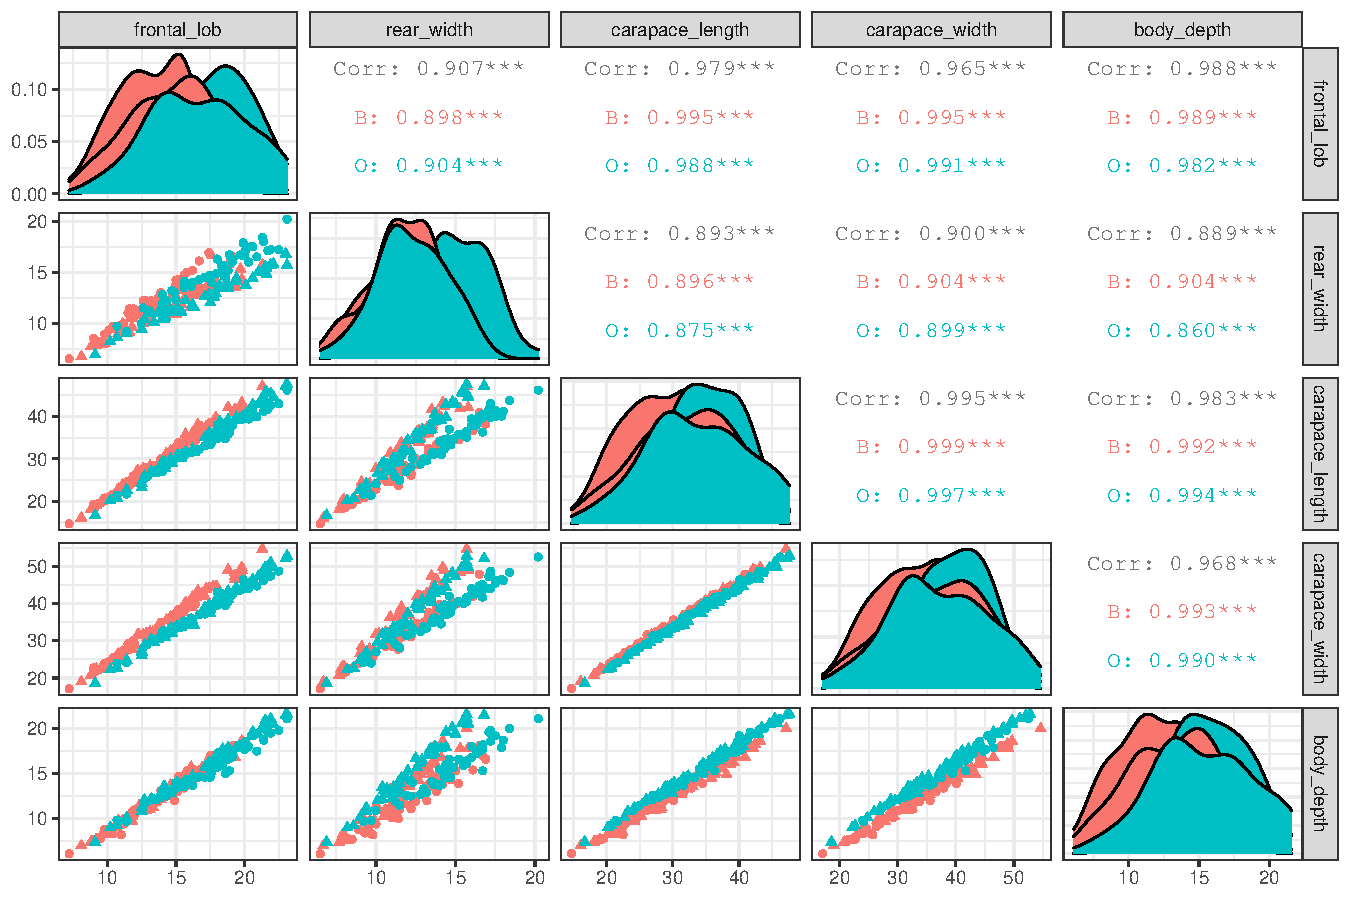
\includegraphics[width=.8\textwidth]{figures/crabs_attributes-1} 

\end{knitrout}
$\rightsquigarrow$ Pairs plot don't help...
\end{frame}

\begin{frame}[fragile]
  \frametitle{Companion data set: 'crabs'}
  \framesubtitle{Correlation matrix}

\begin{knitrout}\scriptsize
\definecolor{shadecolor}{rgb}{0.969, 0.969, 0.969}\color{fgcolor}\begin{kframe}
\begin{alltt}
\hlstd{crabs} \hlopt  \hlkwd{select}\hlstd{(}\hlopt{-}\hlstd{species,} \hlopt{-}\hlstd{sex)} \hlopt \hlkwd{cor}\hlstd{( )} \hlopt \hlkwd{kable}\hlstd{(}\hlstr{'latex'}\hlstd{,} \hlkwc{digits} \hlstd{=} \hlnum{3}\hlstd{)}
\end{alltt}
\end{kframe}
\begin{tabular}{l|r|r|r|r|r}
\hline
  & frontal\_lob & rear\_width & carapace\_length & carapace\_width & body\_depth\\
\hline
frontal\_lob & 1.000 & 0.907 & 0.979 & 0.965 & 0.988\\
\hline
rear\_width & 0.907 & 1.000 & 0.893 & 0.900 & 0.889\\
\hline
carapace\_length & 0.979 & 0.893 & 1.000 & 0.995 & 0.983\\
\hline
carapace\_width & 0.965 & 0.900 & 0.995 & 1.000 & 0.968\\
\hline
body\_depth & 0.988 & 0.889 & 0.983 & 0.968 & 1.000\\
\hline
\end{tabular}


\end{knitrout}

\bigskip

\alert{Very high correlation!}
\begin{itemize}
 \item much redundancy?
 \item hidden factor?
\end{itemize}
$\rightsquigarrow$ dimension reduction might help
\end{frame}

\begin{frame}[fragile]
  \frametitle{Another example: 'snp'}
  \framesubtitle{Genetics variant in European population}

\begin{block}{Description: \textcolor{black}{\it medium/large data, high-dimensional}}
500, 000 Genetics variants (SNP -- Single Nucleotide Polymorphism) for  3000 individuals
(1 meter $\times$ 166 meter (height $\times$ width)
\end{block}

\begin{multicols}{2}
  \begin{itemize}
  \item SNP : 90 \% of human genetic variations
  \item coded as 0, 1 or 2 (10, 1 or 2 allel different against the population reference)
  \end{itemize}

  \begin{figure}
    \centering
     \includegraphics[height=4cm]{SNP}   
    \caption{SNP (wikipedia)}
  \end{figure}
\end{multicols}

\end{frame}

\begin{frame}
  \frametitle{Summarize 500,000 variables in 2}

  \begin{figure}
    \centering
      \includegraphics[height=6cm]{geneMirrorGeography}
    \caption{PCA output {\tiny source: Nature "Gene  Mirror Geography Within  Europe", 2008}}
  \end{figure}

  $\rightsquigarrow$ How much information is lost?

\end{frame}


\begin{frame}
\frametitle{Theoretical argument: dimensionality Curse}

\begin{block}{High Dimension Geometry Curse}
\begin{itemize}
\item Folks theorem: In high dimension, everyone is alone.
\item Theorem: If $\bx_1,\ldots, \bx_n$ in the
hypercube of dimension $d$  such
that their coordinates are i.i.d then
\begin{align*}
\mspace{-20mu} d^{-1/p} \left( \max \|\bx_i-\bx_{i'}\|_p - \min \|\bx_i-\bx_{i'}\|_p
\right)  &= 0 + O\left(\sqrt{\frac{\log n}{d}}\right)\\
\frac{\max \|\bx_i-\bx_{i'}\|_p}{\min \|\bx_i-\bx_{i'}\|_p} &= 1 +
O\left(\sqrt{\frac{\log n}{d}}\right).
\end{align*}
\end{itemize}
\end{block}

  $\rightsquigarrow$ When $d$ is large, all the points are almost equidistant\\

  Hopefully, the data \alert{\bf are not really leaving in $d$} dimension (think of the SNP example)

\end{frame}

\begin{frame}[label=DimensionReduction]
  \frametitle{Dimension reduction: general goals}

  \paragraph{Main objective:} find a \alert{\bf low-dimensional representation} that captures the "essence" of (high-dimensional) data

  \vfill

  \begin{block}{Application in Machine Learning}
  \alert{Preprocessing, Regularization}
  \begin{itemize}
    \item Compression, denoising,  anomaly detection
    \item Reduce overfitting in supervised learning
  \end{itemize}
  \end{block}

\vfill

  \begin{block}{Application in Statistics/Data analysis}
    \alert{Better understanding of the data}
    \begin{itemize}
      \item descriptive/exploratory methods
      \item visualization (difficult to plot and interpret $> 3d$!)
    \end{itemize}
  \end{block}

\end{frame}

\begin{frame}
  \frametitle{Dimension reduction: problem setup}

    \begin{block}{Settings}
      \begin{itemize}
        \item \alert{Training data } : $\mathcal{D}=\{\bx_1,\ldots,\bx_n\} \in \Rset^d$,   (i.i.d.)
        \item Space $\Rset^d$ of possibly high dimension $(n \ll d)$
      \end{itemize}
    \end{block}

    \vfill
    
    \begin{block}{Dimension Reduction Map}
       Construct a map $\Phi$ from the space $\Rset^{d}$ into a space $\Rset^{d'}$ of \alert{smaller dimension}:
      \begin{align*}
          \Phi:\quad & \Rset^d \to \Rset^{d'}, d' \ll d\\
                     & \bx \mapsto \Phi(\bx)
      \end{align*}
    \end{block}
    
\end{frame}
 
\begin{frame}
  \frametitle{How should we design/construct $\Phi$?}

  \paragraph{Criterion}
  \begin{itemize}
    \item \alert{\bf Geometrical approach}
    \item Reconstruction error
    \item Relationship preservation
  \end{itemize}

  \vfill
  
  \paragraph{Form of the map $\Phi$}
  \begin{itemize}
    \item \alert{\bf Linear} or non-linear ?
    \item tradeoff between \alert{\bf interpretability} and versatility ?
    \item tradeoff between high or \alert{\bf low} computational resource
  \end{itemize}

\end{frame}


%% ====================================================================
\part{Principal Component Analysis}
%% ====================================================================
\begin{frame}
  \partpage
\end{frame}

\begin{frame}
  \frametitle{Some references\dots}
  \framesubtitle{\dots biased choices!}
  
    \begin{thebibliography}{99}
      \setbeamertemplate{bibliography item}[book]

    \bibitem[ACP]{ACP} Analyse en composantes principales, \alert{Course AgroParisTech}
    \newblock \textcolor{black}{Carine Ruby, Stéphane Robin}
    \newblock {\tiny\url{http://www.agroparistech.fr/IMG/pdf/AnalyseComposantesPrincipales-AgroParisTech.pdf}}

    \bibitem[husson]{husson} Exploratory Multivariate Analysis by Example using R,
    \newblock \textcolor{black}{Husson, Le, Pages, 2017.}
    \newblock Chapman \& Hall

    \bibitem[pages]{pages} Multiple Factor Analysis by Example using R,
    \newblock \textcolor{black}{J. Pagès 2015.}
    \newblock CRC Press

    \bibitem[ELS]{ELS} An Introduction to Statistical Learning
    \newblock \textcolor{black}{G. James, D. Witten, T. Hastie and R. Tibshirani}
    \newblock {\tiny\url{http://faculty.marshall.usc.edu/gareth-james/ISL/}}

    \end{thebibliography}

\end{frame}

\begin{frame}
  \frametitle{PCA and classical Linear methods}
  
  \paragraph{\bf Principal component Analysis (PCA) is for continuous data}

  \begin{block}{Non continuous data}
  \begin{itemize}
    \item Correspondence analysis (CA): contingency table \medskip
    \item Multiple correspondence analysis (MCA): categorical data \medskip
    \item Multiple factor analysis (MFA): multi-table, array data 
  \end{itemize}
  $\rightsquigarrow$ Basic \alert{adaptations that build on PCA} to deal with non-continuous data\\
  $\rightsquigarrow$ smart encoding of non-continuous data to continuous ones
  \end{block}

  \vfill
  
  \begin{center}
    \alert{\bf We will focus on PCA}, as the mother or most linear (and non-linear) methods.
  \end{center}
  
\end{frame}

\begin{frame}[fragile]
  \frametitle{The data matrix}

  The data set is a $n\times d$ matrix  $\bX = (x_{ij})$ with values in $\Rset$:
  \begin{itemize}
    \item each row $\bx_i$ represents an individual/observation
    \item each col $\bx^j$ represents a variable/attribute
  \end{itemize}

\begin{knitrout}\scriptsize
\definecolor{shadecolor}{rgb}{0.969, 0.969, 0.969}\color{fgcolor}\begin{kframe}
\begin{alltt}
\hlstd{crabs} \hlopt \hlkwd{head}\hlstd{(}\hlnum{6}\hlstd{)} \hlopt \hlstd{knitr}\hlopt{::}\hlkwd{kable}\hlstd{(}\hlstr{"latex"}\hlstd{)}
\end{alltt}
\end{kframe}
\begin{tabular}{l|l|r|r|r|r|r}
\hline
species & sex & frontal\_lob & rear\_width & carapace\_length & carapace\_width & body\_depth\\
\hline
B & M & 8.1 & 6.7 & 16.1 & 19.0 & 7.0\\
\hline
B & M & 8.8 & 7.7 & 18.1 & 20.8 & 7.4\\
\hline
B & M & 9.2 & 7.8 & 19.0 & 22.4 & 7.7\\
\hline
B & M & 9.6 & 7.9 & 20.1 & 23.1 & 8.2\\
\hline
B & M & 9.8 & 8.0 & 20.3 & 23.0 & 8.2\\
\hline
B & M & 10.8 & 9.0 & 23.0 & 26.5 & 9.8\\
\hline
\end{tabular}


\end{knitrout}

\end{frame}

\begin{frame}
  \frametitle{Objectives}
  
\paragraph{Individual/Observations}
  
  \begin{itemize}
    \item similarity between observations with respect to all the variables 
    \item Find pattern ($\sim$ partition) between individuals
  \end{itemize}

\vfill

\paragraph{Variables} 
  
  \begin{itemize}
  \item linear relationships between variables 
  \item visualization of the correlation matrix
  \item find synthetic variables
  \end{itemize}

\vfill

\paragraph{Link between the two}
  
  \begin{itemize}
    \item characterization of the groups of individuals with variables
    \item specific observations to understand links between variables
  \end{itemize}

\end{frame}


%% ==========================================================================
%% Background: high-school algebra
%% ==========================================================================
%% \input{background_algebra}

%% ==========================================================================
%% Geometric point of View
%% ==========================================================================

%% ==========================================================================
\section{Geometric approach to PCA}
%% ==========================================================================

\begin{frame}[fragile]
  \frametitle{The data matrix}

  The data set is a $n\times d$ matrix  $\bX = (x_{ij})$ with values in $\Rset$:
  \begin{itemize}
    \item each row $\bx_i$ represents an individual/observation
    \item each col $\bx^j$ represents a variable/attribute
  \end{itemize}

  \begin{equation*}
    \bX = \bordermatrix{%
           ~ & \bx^1  & \bx^2  &  \dots & \bx^j   & \dots & \bx^d  \cr
    \bx_1  & x_{11} & x_{12} &  \dots & x_{1j} & \dots & x_{1d}  \cr
    \bx_2  & x_{21} & x_{22} &  \dots & x_{2j} & \dots & x_{2d}  \cr
    \vdots & \vdots & \vdots & \vdots & \vdots & \vdots & \vdots  \cr
    \bx_i  & x_{i1} & x_{i2} &  \dots x_{ij} & \dots & x_{id} \cr
    \vdots & \vdots & \vdots & \vdots & \vdots & \vdots & \vdots  \cr
    \bx_n  & x_{n1} & x_{n2} &  \dots x_{nj} & \dots & x_{nd} \cr
    }
  \end{equation*}

\begin{knitrout}\scriptsize
\definecolor{shadecolor}{rgb}{0.969, 0.969, 0.969}\color{fgcolor}\begin{kframe}
\begin{alltt}
\hlstd{crabs} \hlopt \hlkwd{head}\hlstd{(}\hlnum{3}\hlstd{)} \hlopt \hlstd{knitr}\hlopt{::}\hlkwd{kable}\hlstd{(}\hlstr{"latex"}\hlstd{)}
\end{alltt}
\end{kframe}
\begin{tabular}{l|l|r|r|r|r|r}
\hline
species & sex & frontal\_lob & rear\_width & carapace\_length & carapace\_width & body\_depth\\
\hline
B & M & 8.1 & 6.7 & 16.1 & 19.0 & 7.0\\
\hline
B & M & 8.8 & 7.7 & 18.1 & 20.8 & 7.4\\
\hline
B & M & 9.2 & 7.8 & 19.0 & 22.4 & 7.7\\
\hline
\end{tabular}


\end{knitrout}

\end{frame}

\begin{frame}
  \frametitle{Cloud of observation in $\Rset^d$}

  Individuals can be represented in the \alert{variable space $\Rset^d$} as a point cloud

  \begin{columns}
    \begin{column}{.5\textwidth}
      \begin{figure}      
      \includegraphics[width=.6\textwidth]{cloud_centering}
      \vspace{-.25cm}
      \caption{Example in $\Rset^3$}
      \end{figure}      
    \end{column}

  \begin{column}{.5\textwidth}
    \begin{block}{Center of Inertia}
      (or barycentrum, or empirical mean)
      \[ \bar{\bx} = \frac{1}{n} \sum _{i=1}^n \bx_i = 
      \begin{pmatrix}
        \sum _{i=1}^n x_{i1}/n \\
        \sum _{i=1}^n x_{i2}/n \\
        \vdots\\
        \sum _{i=1}^n x_{id} /n
      \end{pmatrix}
      \]
    \end{block}
  \end{column}
  \end{columns}

  We center the cloud $\bX$ around $\bx$ denote this by $\bX^c$
  \begin{equation*}
    \bX^c = \begin{pmatrix}
    x_{11} - \bar{x}_1 &   \dots & x_{1j}  - \bar{x}_j & \dots  & x_{1d} - \bar{x}_d   \cr
              \vdots   &  \vdots & \vdots              & \vdots & \vdots  \cr
    x_{i1} - \bar{x}_1 &   \dots & x_{ij} - \bar{x}_j  & \dots  & x_{id}  - \bar{x}_d \cr
              \vdots   &  \vdots & \vdots              & \vdots & \vdots  \cr
    x_{n1} - \bar{x}_1 &  \dots  & x_{nj} - \bar{x}_j  & \dots  & x_{nd}  - \bar{x}_d \cr
    \end{pmatrix}
  \end{equation*}

\end{frame}

\begin{frame}
  \frametitle{Inertia and Variance}

\begin{block}{Total Inertia: \textcolor{black}{distance of the individuals to the center of the cloud}}
  \[
      I_T = \frac{1}{n}\sum_{i=1}^n \sum_{j=1}^d  (x_{ij}- \bar{x}_{j}) ^2 
      = \frac{1}{n}\sum_{i=1}^n \|\bx_i - \bar{\bx} \|^2  
      = \frac{1}{n}\sum_{i=1}^n \distance^2 (\bx_i,\bar{\bx})
    \]
\end{block}

  \begin{block}{$I_T$ is proportional to the total variance}
  Let $\hat{\bSigma}$ be the empirical variance-covariance matrix
\[
      I_T = \frac{1}{n}\sum_{j=1}^p  \sum_{i=1}^n (x_{ij}- \bar{x}_{j}) ^2 
      = \sum_{j=1}^n \frac{1}{n}\|\bx^j - \bar{x}_{j} \|^2
      = \sum_{j=1}^n \var(\bx^j) = \trace{\hat{\bSigma}}
\]
\end{block}

\begin{itemize}
  \item[$\rightsquigarrow$] \alert{Good representation has large inertia} (much variability)
  \item[$\rightsquigarrow$] \alert{Large dispertion $\sim$ Large distances between points}
\end{itemize}
  
\end{frame}

\begin{frame}
  \frametitle{Inertia with respect to an axix}

  The Inertia of the cloud wrt axe $\Delta$ is the sum of the distances between all points and their orthogonal projection on $\Delta$.
  \begin{equation*}
    \begin{aligned}
      I_\Delta = \frac{1}{n}\sum_{i=1}^n \distance^2(\bx_i, \Delta)
      \end{aligned}
  \end{equation*}

  \begin{figure}
    \includegraphics[width=.7\textwidth]{proj_axis}
    \caption{Projection of $\bx_i$ onto a line $\Delta$ passing through $\bar\bx$}
  \end{figure}

\end{frame}

\begin{frame}
  \frametitle{Decomposition of total Inertia (1)}
  
  Let $\Delta^\bot$ the orthogonal subspace $\Delta$  is $\Rset^n$

  \includegraphics[width=.5\textwidth]{supp_spaces}

  \begin{block}{Theorem (Huygens)}
    A consequence of the above (Pythagoras Theorem) is the decomposition of the following total inertia:
      \begin{equation*}
        I_T = I_{\Delta} + I_{\Delta^\bot}
      \end{equation*}
    \alert{By projecting the cloud $\bX$ onto $\Delta$, with loss the inertia measured by $\Delta^\bot$}
    \end{block}
        
\end{frame}

\begin{frame}
  \frametitle{Decomposition of total Inertia (2)}
  
  Consider only subspaces with dimension $1$ (that is, lines or axes). We can decompose $\Rset^p$ as the sum of $p$ othogonal axis. 
  
  \begin{equation*}
    \Rset^p = \Delta_1 \oplus \Delta_2 \oplus \dots \oplus \Delta_p
  \end{equation*}
  \alert{$\rightsquigarrow$ These axes form a new basis for representing the point cloud.}

  \begin{block}{Theorem (Huygens)}
    \begin{equation*}
      I_{T} = I_{\Delta_1} + I_{\Delta_2} + \dots + I_{\Delta_p}
    \end{equation*}
  \end{block}
  
\end{frame}

%% ==========================================================================
%% Principal axes by variance maximization
%% ==========================================================================

%% ==========================================================================
\section{Principal axes and variance maximization}
%% ==========================================================================

\begin{frame}
  \frametitle{Finding the best axis (1)}

  \begin{block}{Definition of the problem}
    \begin{itemize}
      \item The best axis $\Delta_1$ is the "closest" to the point cloud
      \item Inertia of $\Delta_1$ measures the distance between the data and $\Delta_1$
      \item $\Delta_1$ is defined by the director vector $\bu_1$, such as $\| \bu_1 \| = 1$
      \item $\Delta_1^\bot$ is defined by the normal  vector $\bu_1$, such as $\| \bu_1 \| = 1$
    \end{itemize}
    \alert{$\rightsquigarrow$ The best axis $\Delta_1$ is the one with the minimal Inertia.}
  \end{block}
  
\end{frame}

\begin{frame}
  \frametitle{Finding the best axis (2)}

  \begin{block}{Stating the optimization problem}
    Since $\Delta_1 \oplus \Delta_1^\bot = \Rset^p$ and $I_T = I_{\Delta_1} + I_{\Delta_1^\bot}$ , then
    \begin{equation*}
        \minimize_{\bu \in \Rset^p: \|\bu\| = 1} I_{\Delta_1} \Leftrightarrow \maximize_{\bu \in \Rset^p: \|\bu\| = 1} I_{\Delta_1^\bot}
    \end{equation*} 
  \end{block}  
  
  \includegraphics[width=.7\textwidth]{minimum_inertia}
  
\end{frame}

\begin{frame}
  \frametitle{Finding the best axis (3)}

\begin{columns}
  \begin{column}{.5\textwidth}
  \begin{block}{Stating the problem (algebraically)}
    Find $\bu_1; \|\bu_1 \|=1$ that minimizes
    \begin{equation*}
      \begin{aligned}
        I_{\Delta_1^\bot} & = \frac{1}{n}\sum_{i=1}^n \distance(\bx_i,\Delta_1^\bot)^2 \\ 
        & = \frac{1}{n}\sum_{i=1}^n \bu_1^\top (\bx_i - \bar{\bx})(\bx_i - \bar{\bx})^\top \bu_1 \\
        & = \bu_1^\top \left( \sum_{i=1}^n \frac{1}{n}(\bx_i - \bar{\bx})(\bx_i - \bar{\bx})^\top \right)  \bu_1 \\
        & = \bu_1^\top \hat{\bSigma}  \bu_1
      \end{aligned}
    \end{equation*} 
  \end{block}  
  \end{column}
  \begin{column}{.45\textwidth}
  \begin{figure}
    \includegraphics[width=.9\textwidth]{solving_inertia}
    \caption{Geometrical insight}
  \end{figure}
  \end{column}
\end{columns}
  
\end{frame}

\begin{frame}
  \frametitle{Finding the best axis (4)}

  We solve a simple constraint maximization problem with the method of Lagrange multipliers:
  
  \begin{equation*}
    \maximize_{\bu_1: \|\bu_1\| = 1 } \bu_1^\top \hat\bSigma \bu_1 \Leftrightarrow \maximize_{\bu_1\in\Rset^p, \lambda_1 > 0} \bu_1^\top \hat\bSigma \bu_1 - \lambda_1 (\|\bu_1\| - 1)
  \end{equation*}
  
  By straightforward (vector) differentiation, an using that $\bu_1^\top \bu_1 = 1$
  \begin{equation*}
    \left\{\begin{aligned}
      2\hat\bSigma \bu_1 - 2\lambda_1 \bu_1 & = 0 \\  
      \bu_1^\top \bu_1 - 1 & = 0 \\  
    \end{aligned}\right. \Leftrightarrow
    \left\{\begin{aligned}
      \hat\bSigma \bu_1 & = \lambda_1 \bu_1  \\  
      \bu_1^\top \hat\bSigma \bu_1 & = \lambda_1 \bu_1^\top \bu_1 = \lambda_1 = I_{\Delta_1}^\bot \\  
    \end{aligned}\right.
  \end{equation*}
  
  \begin{itemize} 
     \item $\bu_1$ is the first eigen vector of $\hat{\bSigma}$
     \item $\lambda_1$ is the first eigen value of $\hat{\bSigma}$
   \end{itemize} 
  
  $\rightsquigarrow$ \alert{\bf $\Delta_1$ is defined by the first eigen vector of $\hat\bSigma$}\\
  $\rightsquigarrow$ \alert{\bf Variance "carried" by $\Delta_1$ is equal to the largest eigen value of $\hat\bSigma$}
  
\end{frame}

\begin{frame}
  \frametitle{Finding the following axes}

  \begin{block}{Second best axis}
    Find $\Delta_2$ with dimension 1, director vector $\bu_2$ orthogonal to $\Delta_1$ solving
    \begin{equation*}
        \maximize_{\bu_2 \in \Rset^p} I_{\Delta_2^\bot} = \bu_2^\top \hat{\bSigma}\bu_2, \quad \text{with } \|\bu_2\| = 1, \bu_1^\top \bu_2 = 0.
    \end{equation*} 
  $\rightsquigarrow$ $\bu_2$ is the second eigen vector of $\hat\bSigma$ with eigen value $\lambda_2$
  \end{block}
  
  \vfill
  \pause
  
  \begin{block}{And so on!}
    PCA is roughly a matrix factorisation problem 
    \begin{equation*}
      \hat\bSigma = \bU \boldsymbol\Lambda \bU^\top, \quad
      \bU = \begin{pmatrix}
      \bu_1 & \bu_2, & \dots & \bu_p
      \end{pmatrix}, \quad \boldsymbol\Lambda = \diag(\lambda_1, \dots, \lambda_p)
    \end{equation*}
    \hspace{-.5cm}
  \begin{itemize}
    \item $\bU$ is an orthogonal matrix of normalized eigen vectors.
    \item $\boldsymbol\Lambda$ is diagonal matrix of  ordered eigen values.
  \end{itemize}
  \end{block}
\end{frame}

\begin{frame}
  \frametitle{Interpretation in $\Rset^p$}
    
  $\bV$ describes a new orthogonal basis and a rotation of data in this basis\\
  $\rightsquigarrow$ PCA is an appropriate rotation on axes that maximizes the variance

  \begin{equation*}
    \left\{\begin{array}{ccccc}
      \Delta_1 & \oplus & \dots & \oplus & \Delta_p \\
      \bu_1 & \bot & \dots & \bot & \bu_2 \\
      \lambda_1 & > & \dots & > & \lambda_p \\
      I_{\Delta_1^\bot} & > & \dots & > & I_{\Delta_p^\bot} \\
    \end{array}\right.
  \end{equation*}

  \includegraphics[width=.6\textwidth]{rotation}
\end{frame}

%% ==========================================================================
%% Representation and interpretation
%% ==========================================================================

\section{Representation and interpretation}

\subsection{Quality of the reconstruction}

\begin{frame}
  \frametitle{Contribution of each axis and quality of the representation}
  
  $\Delta_k$ is carrying inertia/variance defined by its orthogonal, thus 
  \begin{equation*}
      I_T = I_{\Delta_1^\bot} + \dots + I_{\Delta_p^\bot} = \lambda_1 + \dots + \lambda_p
  \end{equation*}

  \begin{block}{Relative contribution of axis $k$}<2->
    \vspace{-.5cm}
  \[ 
    \mathrm{contrib}(\Delta_k) = \frac{\lambda_k}{\sum_{k=1}^p\lambda_j} = \frac{\lambda_k}{\trace{\hat\bSigma}} \times 100 
  \]
    $^\rightsquigarrow$ \alert{Percentage of explained inertia/variance explained}
  \end{block}

  \begin{block}{Global quality of the representation on the first $k$ axes}<3->
    \vspace{-.5cm}
  \[ 
    \mathrm{contrib}(\Delta_1,\dots,\Delta_k) = \frac{\lambda_1 + \dots + \lambda_k}{\trace{\hat\bSigma}}  \times 100 
  \]
    A few axes may explain a large proportion of the total variance.\\
    $\rightsquigarrow$ \alert{This paves the way for dimension reduction} 
  \end{block}
  
\end{frame}

\begin{frame}[fragile]
  \frametitle{Scree plot: 'crabs'}

\begin{knitrout}\scriptsize
\definecolor{shadecolor}{rgb}{0.969, 0.969, 0.969}\color{fgcolor}\begin{kframe}
\begin{alltt}
\hlstd{crabs_pca} \hlkwb{<-} \hlkwd{select}\hlstd{(crabs,} \hlopt{-}\hlstd{species,} \hlopt{-}\hlstd{sex)} \hlopt \hlstd{FactoMineR}\hlopt{::}\hlkwd{PCA}\hlstd{(}\hlkwc{graph} \hlstd{=} \hlnum{FALSE}\hlstd{)}
\hlkwd{fviz_eig}\hlstd{(crabs_pca)}
\end{alltt}
\end{kframe}
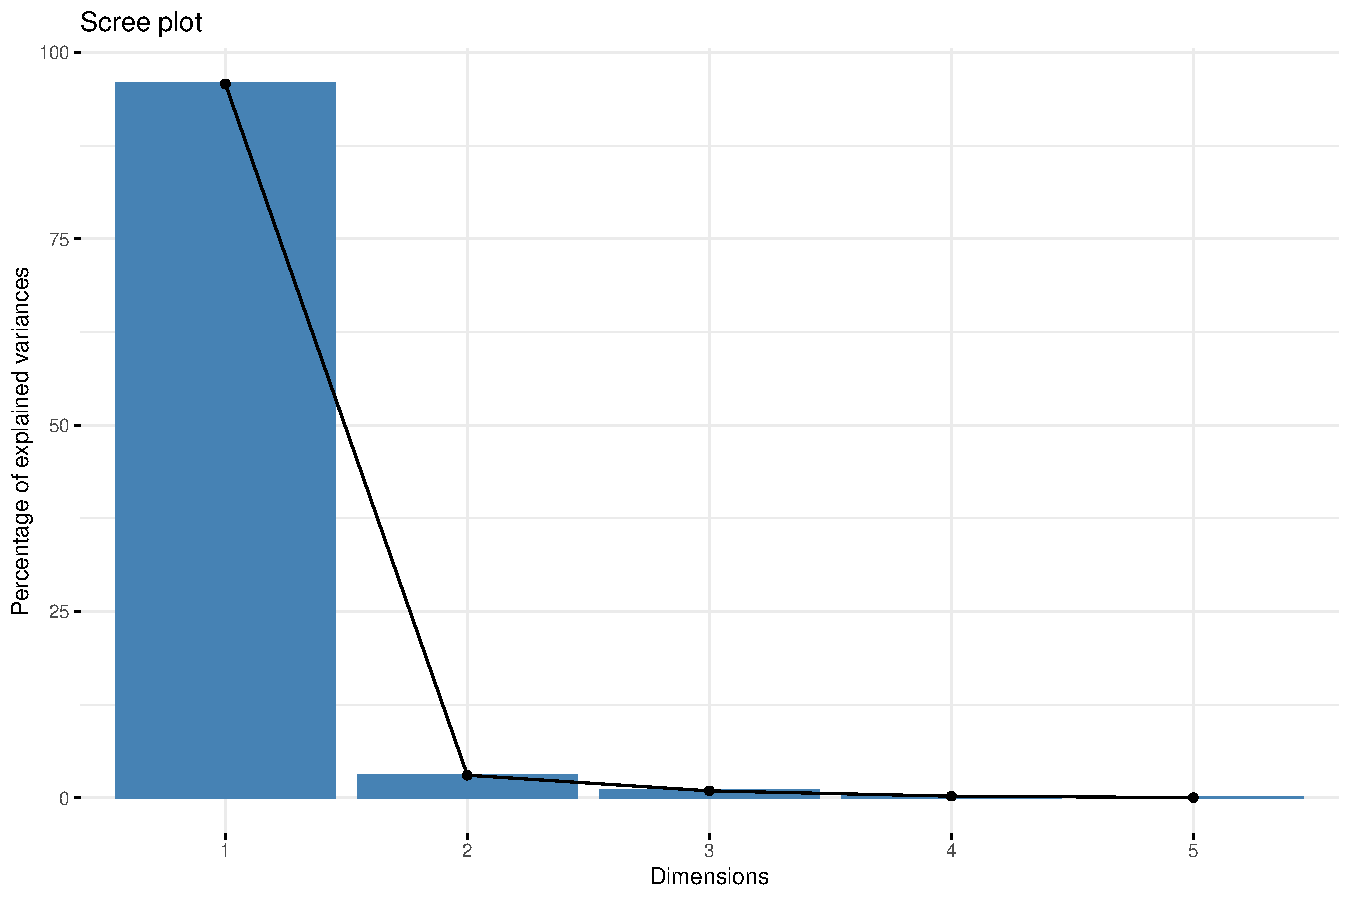
\includegraphics[width=.8\textwidth]{figures/pca_crabs_screeplot-1} 

\end{knitrout}

$\rightsquigarrow$  We will see during labs why everything is carried by the first axis

\end{frame}

\subsection{Individuals point of view}

\begin{frame}
  \frametitle{Individuals: representation in the new basis}

  \begin{block}{Projection of point $\bx_i$ axis $k$}
    The projection of $\bx_i$ onto axis $\Delta_k$ is $c_{ik} \bu_k$, with 
    \begin{equation*}
      c_{ik} = \bu_k^\top (\bx_i - \bar{\bx}),
    \end{equation*}
     the coordinate of $i$ in the basis $\bu_k$ (along axis $\Delta_k$).
  \end{block}

  \begin{block}{Coordinates of $i$ in the new basis}
    Coordinates of $i$ in the new basis $\{\bu1, \dots, \bu_d\}$ is thus 
    \begin{equation*}
      \bc_i  = (\bU^\top (\bx_i - \bar{\bx}))^\top = (\bx_i - \bar{\bx})^\top \bU = \bX^c_i \bU, \quad \bc_i \in \Rset^p.
    \end{equation*}

    \begin{itemize}
      \item \alert{$\bU$ are often the called the \textbf{loadings}, or \textbf{weights}}
      \item \alert{$ \bc_i$ are the \textbf{scores} or \textbf{coordinates} in the new space for the individuals}
    \end{itemize}
  \end{block}
\end{frame}


\begin{frame}[fragile]
  \frametitle{Individual visualization: projection in the new basis (1)}

\begin{knitrout}\scriptsize
\definecolor{shadecolor}{rgb}{0.969, 0.969, 0.969}\color{fgcolor}\begin{kframe}
\begin{alltt}
\hlkwd{fviz_pca_ind}\hlstd{(crabs_pca,} \hlkwc{col.ind} \hlstd{=} \hlkwd{paste}\hlstd{(crabs}\hlopt{$}\hlstd{species, crabs}\hlopt{$}\hlstd{sex),} \hlkwc{palette} \hlstd{= pal)}
\end{alltt}
\end{kframe}
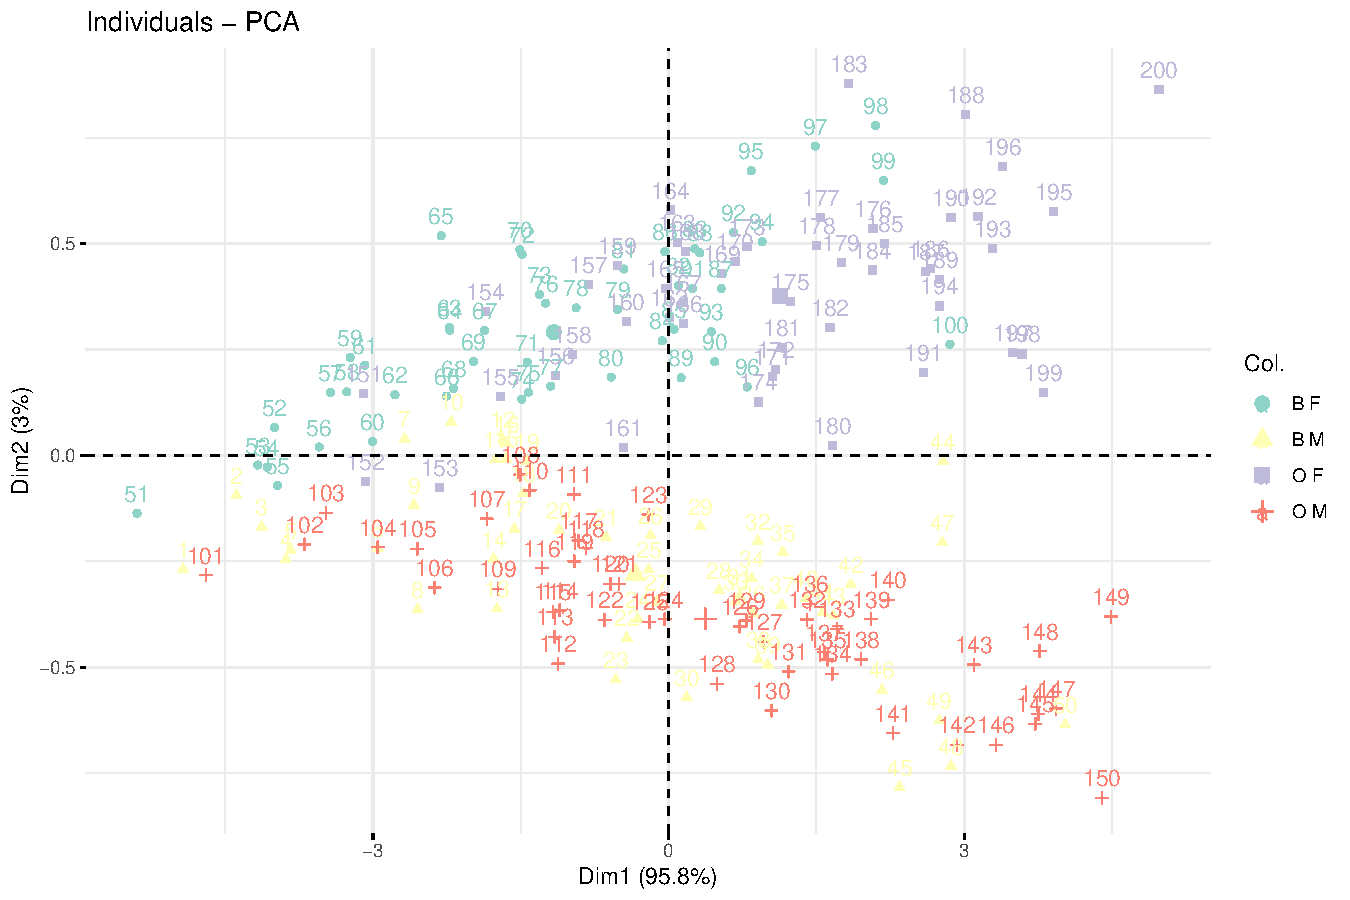
\includegraphics[width=.8\textwidth]{figures/pca_crabs_indmap1-1} 

\end{knitrout}

\end{frame}

\begin{frame}[fragile]
  \frametitle{Individual visualization: projection in the new basis (2)}

\begin{knitrout}\scriptsize
\definecolor{shadecolor}{rgb}{0.969, 0.969, 0.969}\color{fgcolor}\begin{kframe}
\begin{alltt}
\hlkwd{fviz_pca_ind}\hlstd{(crabs_pca,} \hlkwc{axes} \hlstd{=} \hlkwd{c}\hlstd{(}\hlnum{2}\hlstd{,}\hlnum{3}\hlstd{),} \hlkwc{col.ind} \hlstd{=} \hlkwd{paste}\hlstd{(crabs}\hlopt{$}\hlstd{species, crabs}\hlopt{$}\hlstd{sex),} \hlkwc{palette} \hlstd{= pal)}
\end{alltt}
\end{kframe}
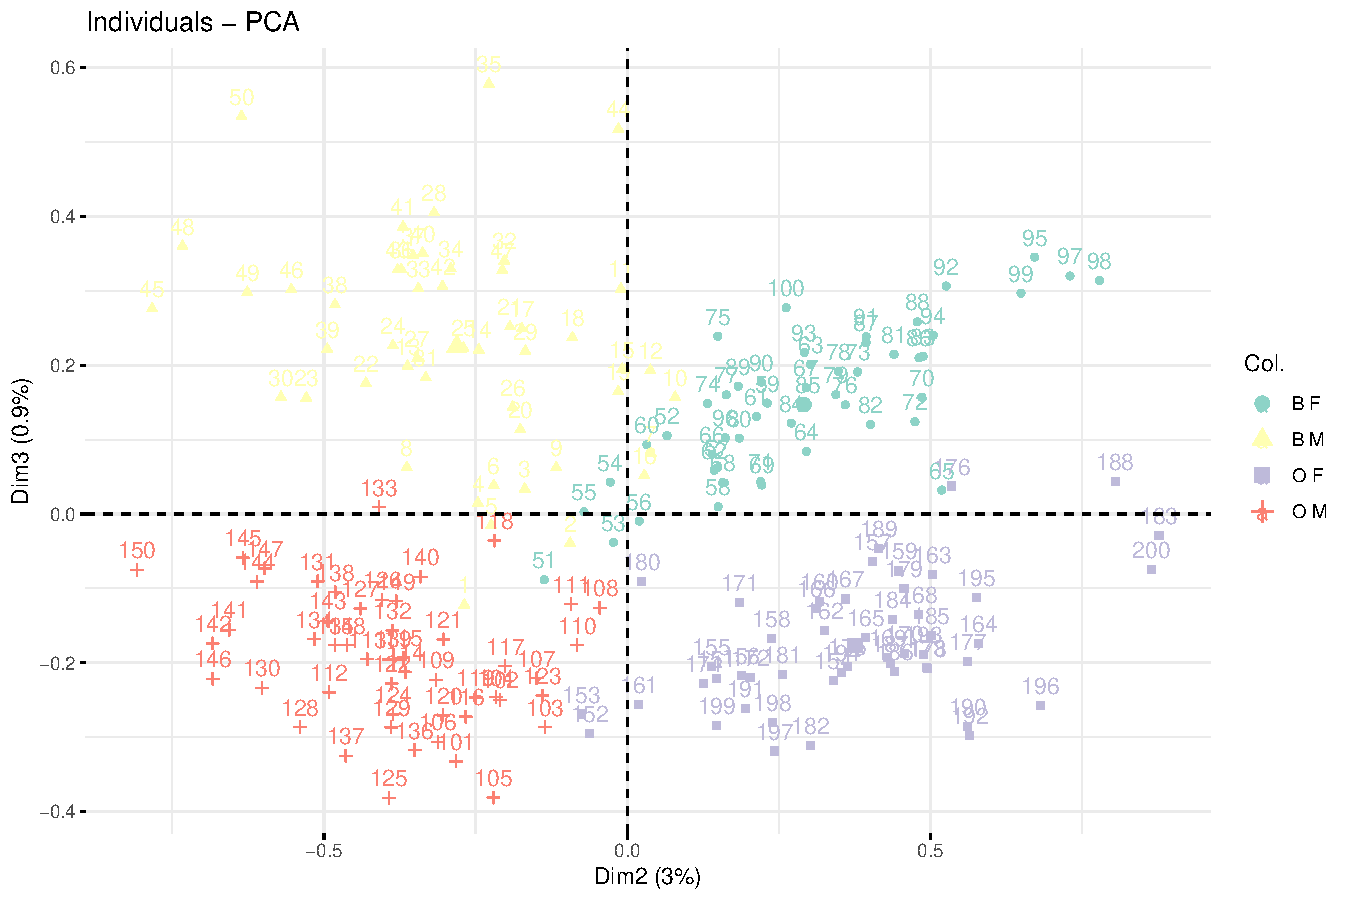
\includegraphics[width=.8\textwidth]{figures/pca_crabs_indmap2-1} 

\end{knitrout}

\end{frame}

\begin{frame}{Warning: about distances after projection}

  \alert{Close projection doesn't mean close individuals!}

  \begin{figure}
    \includegraphics[width = .35\textwidth]{plan_indiv_proche}\\[1ex]
    \includegraphics[width = .35\textwidth]{plan_3d_proche}
    \includegraphics[width = .35\textwidth]{plan_3d_eloigne}
    \includegraphics[width = .35\textwidth]{plan_3d_proche2}
    \includegraphics[width = .35\textwidth]{plan_3d_eloigne2}
    \caption{Same projections but different situations {\tiny (source: E. Matzner)}}

  \end{figure}

 $\rightsquigarrow$ Only work when individuals are well represented in the lower space
\end{frame}

\begin{frame}[fragile]
  \frametitle{Individual: quality of the representation}
  
  \begin{block}{Property}
    \begin{itemize}
      \item  An individual $i$ is well represented by $\Delta_k$ if it is close to this axis.
      \item  In other word, vector $\bx_i - \bar{\bx}$ and $\bu_k$ are close to collinear
    \end{itemize}
  \end{block}
 
     We use the cosine of the angle $\theta_{ik}$ between $\bx_i - \bar{\bx}$ and $\bu_k$ to measure the degree of co-linearity:
     \begin{equation*}
       \cos^2(\theta_{ik}) = \frac{\bigg(\bu_k^\top (\bx_i - \bar{\bx})\bigg)^2}{\|\bx_i - \bar{\bx} \|^2 \xout{\|\bu_k \|^2}}
     \end{equation*}

\begin{knitrout}\scriptsize
\definecolor{shadecolor}{rgb}{0.969, 0.969, 0.969}\color{fgcolor}\begin{kframe}
\begin{alltt}
\hlstd{factoextra}\hlopt{::}\hlkwd{get_pca_ind}\hlstd{(crabs_pca)}\hlopt{$}\hlstd{cos2} \hlopt \hlkwd{head}\hlstd{(}\hlnum{3}\hlstd{)} \hlopt \hlkwd{kable}\hlstd{(}\hlstr{"latex"}\hlstd{)}
\end{alltt}
\end{kframe}
\begin{tabular}{r|r|r|r|r}
\hline
Dim.1 & Dim.2 & Dim.3 & Dim.4 & Dim.5\\
\hline
0.9961694 & 0.0029565 & 0.0006132 & 6.29e-05 & 1.98e-04\\
\hline
0.9994582 & 0.0004598 & 0.0000800 & 1.60e-06 & 5.00e-07\\
\hline
0.9980940 & 0.0016699 & 0.0000663 & 8.50e-05 & 8.48e-05\\
\hline
\end{tabular}


\end{knitrout}
\end{frame}

\begin{frame}[fragile]
  \frametitle{Individual: contribution to an axis}


  \begin{block}{Property}
    \begin{itemize}
      \item Inertia "explained" by $\Delta_k$ is inertia of $\Delta_k^\bot$
      \item $I_{\Delta_k^\bot} = n^{-1}\sum_{i=1}^n \distance^2(\Delta_k^\bot, \bx_i) $
    \end{itemize}
  \end{block}
 
     Contribution of $\bx_i$ to axis $\Delta_k$ is the proportion of variance/inertia carried by individual $i$:
     \begin{equation*}
       \mathrm{contr} (\bx_i) = \frac{n^{-1}\distance^2(\Delta_k^\bot, \bx_i)}{I_{\Delta_k^\bot}} = \frac{\bigg(\bu_k^\top (\bx_i - \bar{\bx})\bigg)^2}{n\lambda_k} 
     \end{equation*}


\begin{knitrout}\scriptsize
\definecolor{shadecolor}{rgb}{0.969, 0.969, 0.969}\color{fgcolor}\begin{kframe}
\begin{alltt}
\hlstd{factoextra}\hlopt{::}\hlkwd{get_pca_ind}\hlstd{(crabs_pca)}\hlopt{$}\hlstd{contr} \hlopt \hlkwd{head}\hlstd{(}\hlnum{3}\hlstd{)} \hlopt \hlkwd{kable}\hlstd{(}\hlstr{"latex"}\hlstd{)}
\end{alltt}
\end{kframe}
\begin{tabular}{r|r|r|r|r}
\hline
Dim.1 & Dim.2 & Dim.3 & Dim.4 & Dim.5\\
\hline
2.535166 & 0.2375409 & 0.1602617 & 0.0688010 & 1.4097141\\
\hline
2.008687 & 0.0291717 & 0.0165027 & 0.0013421 & 0.0027214\\
\hline
1.779751 & 0.0940074 & 0.0121362 & 0.0651696 & 0.4231593\\
\hline
\end{tabular}


\end{knitrout}
  
\end{frame}

\subsection{Variables point of view}

\begin{frame}
  \frametitle{Cloud of variables in $\Rset^n$}
  
  \begin{center}
    \includegraphics[width=.45\textwidth]{nuage_var}
  \end{center}

  Direct equivalence between geometry and statistics (collinearity $\equiv$ correlation) 
  \begin{equation*}
    \cos(\theta_{kl}) = \frac{\langle \bx^k ,\bx^\ell \rangle}{\|\bx^k\| \|\bx^\ell\|} = \rho(\bx^k,\bx^\ell)
  \end{equation*}

\end{frame}

\begin{frame}
  \frametitle{Principal Components}
  
  \begin{block}{Dual representation}
    A symmetric reasoning can be made in $\Rset^n$ for the variables, like with the individuals in $\R^p$.
    
    $\rightsquigarrow$ New axes are linear combinason of the original variables, which can be seen as \alert{\bf new variables} in the new latent space
  \end{block}

  \begin{block}{Principal component}
    It is the linear combinason formed by the orginal variables with weights given by the loadings $\bu_k$
    \begin{equation*}
      \mathbf{f}_{k}  = \sum_{j=1}^p \bu_k (\bx^{j} - \bar{x}_j) = \bX^c \bu_k, \quad \mathbf{f}_k \in \Rset^n
    \end{equation*}
    Sometimes called \alert{"factors"} in  factor analysis, as \alert{latent (hidden) variables}. 
  \end{block}

\end{frame}

\begin{frame}
  \frametitle{Variable representation in the new space}
  
  \begin{block}{Connection with original variables}
    \begin{itemize}
      \item essential for interpretation
      \item answer to the question: how reading the axis of the individual map
      \item use correlation to measure connection to original variable
    \end{itemize}
  \end{block}

  \begin{equation*}
    \var(\mathbf{f}_k) = \frac{1}{n}\var(\bX^c \bu_k) = \bu_k^\top \frac{1}{n}(\bX^c)^\top \bX^c \bu_k =  \bu_k^\top \hat{\bSigma} \bu_k = \lambda_k
  \end{equation*}
  
  \begin{equation*}
    \cov(\mathbf{f}_k, (\bx^j - \bar{x}_j)) = \bu_k \top {\bX^c}^\top \bX^c e_j = \bu_k \lambda_k e_j = \lambda_k \bu_{kj}   
  \end{equation*}

  \begin{equation*}
    \cor(\mathbf{f}_k, (\bx^j - \bar{x}_j)) =  \sqrt{\frac{\lambda_k}{\var(\bx^j)}}\bu_{kj}
  \end{equation*}
  
\end{frame}

\begin{frame}[fragile]
  \frametitle{Variable vizualisation: correlation circle (1)}

\begin{knitrout}\scriptsize
\definecolor{shadecolor}{rgb}{0.969, 0.969, 0.969}\color{fgcolor}\begin{kframe}
\begin{alltt}
\hlkwd{fviz_pca_var}\hlstd{(crabs_pca)}
\end{alltt}
\end{kframe}
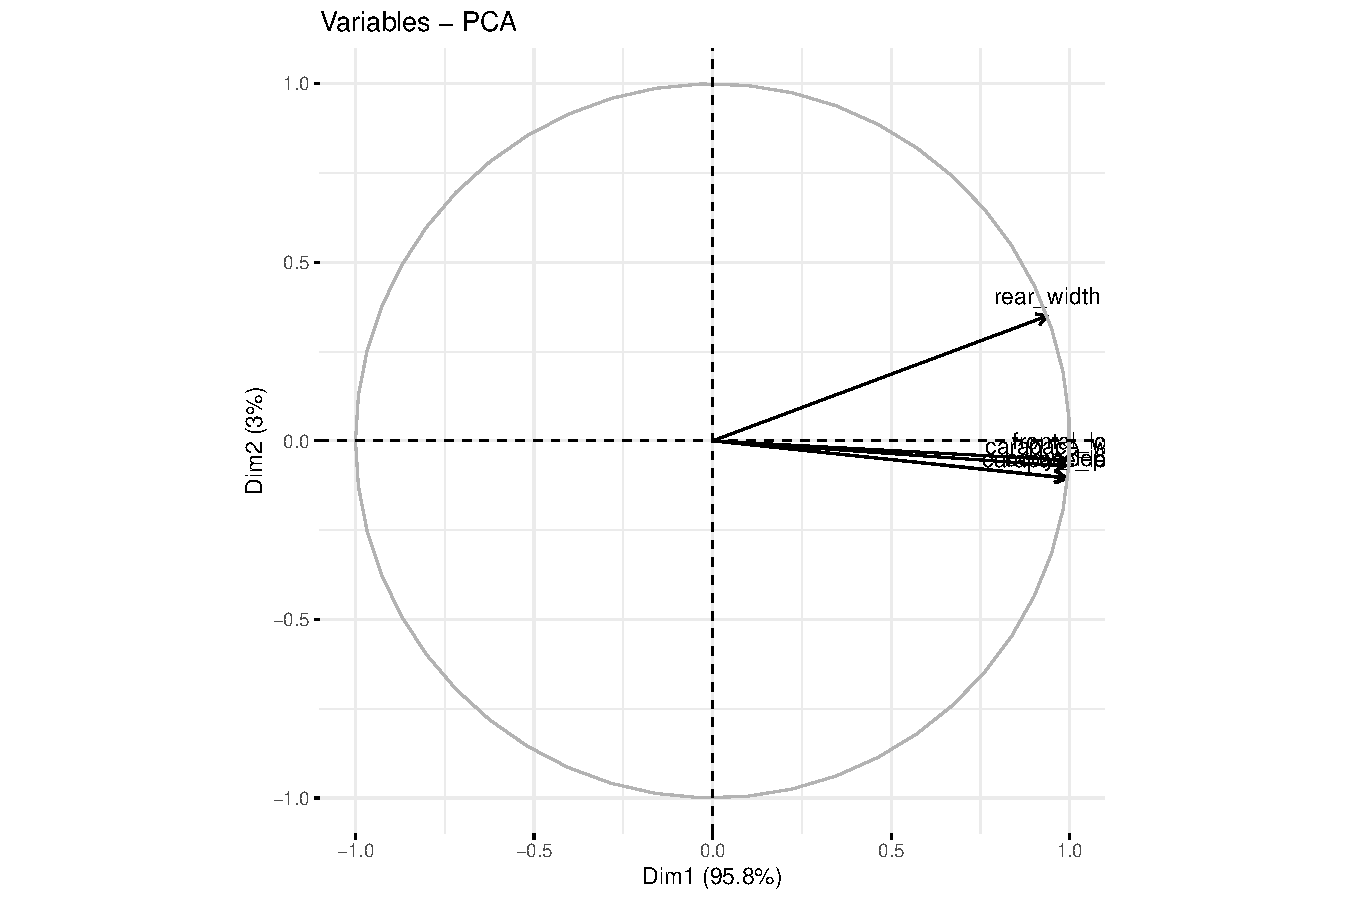
\includegraphics[width=.8\textwidth]{figures/pca_crabs_varmap1-1} 

\end{knitrout}

\end{frame}

\begin{frame}[fragile]
  \frametitle{Variable vizualisation: correlation circle (2)}

\begin{knitrout}\scriptsize
\definecolor{shadecolor}{rgb}{0.969, 0.969, 0.969}\color{fgcolor}\begin{kframe}
\begin{alltt}
\hlkwd{fviz_pca_var}\hlstd{(crabs_pca,} \hlkwc{axes} \hlstd{=} \hlkwd{c}\hlstd{(}\hlnum{2}\hlstd{,}\hlnum{3}\hlstd{))}
\end{alltt}
\end{kframe}
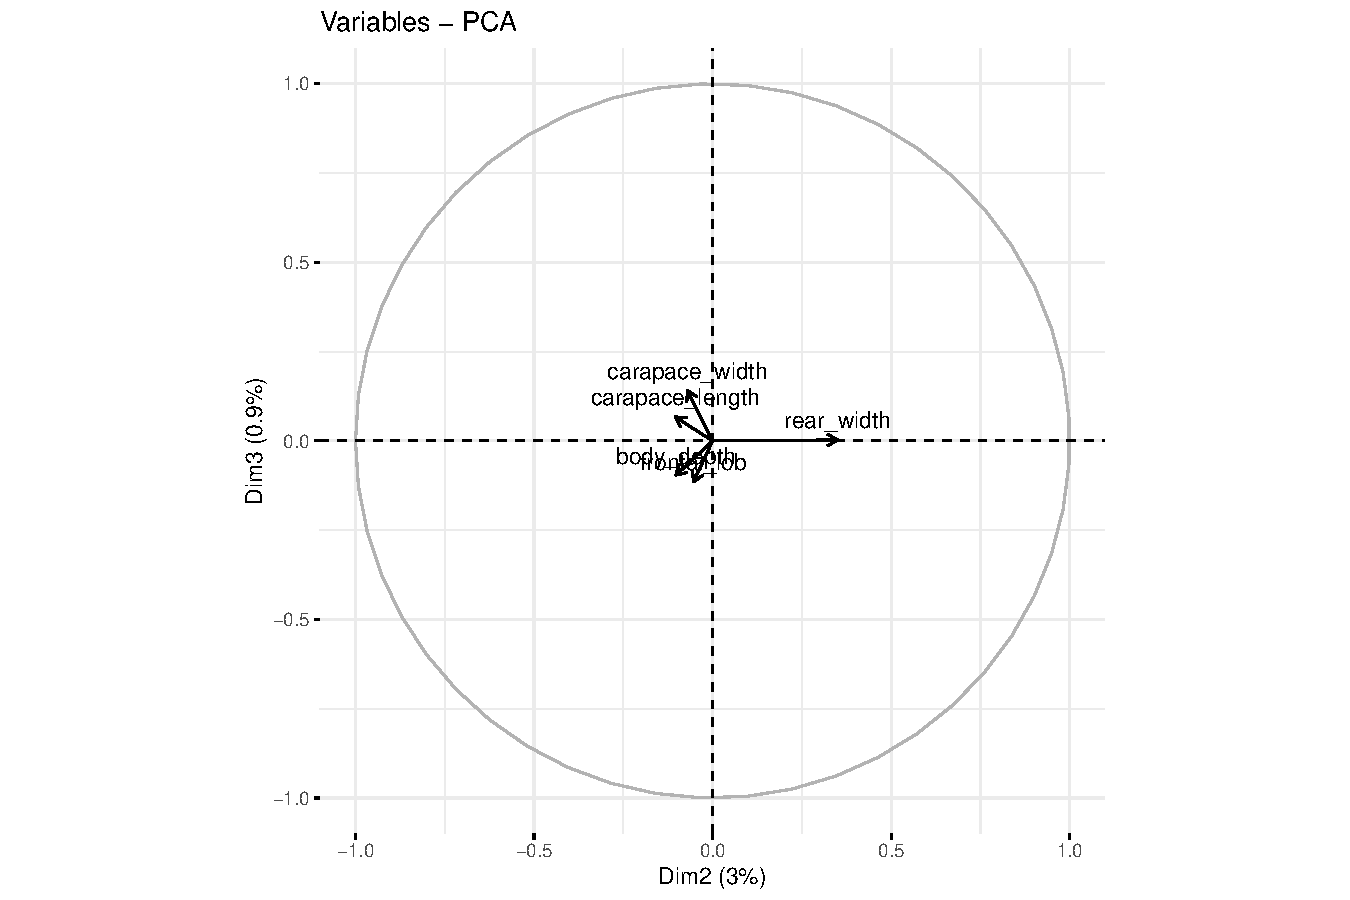
\includegraphics[width=.8\textwidth]{figures/pca_crabs_varmap2-1} 

\end{knitrout}

\end{frame}

\begin{frame}{Warning: about angle after projection}

  \alert{Close projection doesn't mean close variable!}

  \begin{figure}
    \includegraphics[width = .85\textwidth]{proj_var_acp}
    \caption{Same angle but different situations {\tiny (source: J. Josse)}}

  \end{figure}

 $\rightsquigarrow$ Only work when variables are well represented in the latent space
\end{frame}

\begin{frame}[fragile]
  \frametitle{Variable: quality of the representation}

  Same story as for individuals
  \begin{block}{Property}
    \begin{itemize}
      \item  An variable $j$ is well represented by $\Delta_k$ if its projection is close to $\mathbf{f}_k$.
      \item  High collinearity means high absolute correlation and high cosine.
      \item  use cosine to the square of the angle between the original and new variables.
    \end{itemize}
   $\rightsquigarrow$ The projection of $j$ must be close to the boundardy of the correlation circle
  \end{block}
 
\begin{knitrout}\scriptsize
\definecolor{shadecolor}{rgb}{0.969, 0.969, 0.969}\color{fgcolor}\begin{kframe}
\begin{alltt}
\hlstd{factoextra}\hlopt{::}\hlkwd{get_pca_var}\hlstd{(crabs_pca)}\hlopt{$}\hlstd{cos2} \hlopt \hlkwd{head}\hlstd{(}\hlnum{3}\hlstd{)} \hlopt \hlkwd{kable}\hlstd{(}\hlstr{"latex"}\hlstd{)}
\end{alltt}
\end{kframe}
\begin{tabular}{l|r|r|r|r|r}
\hline
  & Dim.1 & Dim.2 & Dim.3 & Dim.4 & Dim.5\\
\hline
frontal\_lob & 0.9785672 & 0.0028712 & 0.0131372 & 0.0054085 & 0.0000159\\
\hline
rear\_width & 0.8775551 & 0.1223552 & 0.0000067 & 0.0000780 & 0.0000051\\
\hline
carapace\_length & 0.9835409 & 0.0109140 & 0.0044722 & 0.0000000 & 0.0010728\\
\hline
\end{tabular}


\end{knitrout}

\end{frame}

\begin{frame}[fragile]
  \frametitle{Variable: contribution to an axis}
  
  Similarly to individuals, we can measure the contribution of the original variables to the construction of the new ones.
  
\begin{knitrout}\scriptsize
\definecolor{shadecolor}{rgb}{0.969, 0.969, 0.969}\color{fgcolor}\begin{kframe}
\begin{alltt}
\hlstd{factoextra}\hlopt{::}\hlkwd{get_pca_var}\hlstd{(crabs_pca)}\hlopt{$}\hlstd{contr} \hlopt \hlkwd{kable}\hlstd{(}\hlstr{"latex"}\hlstd{)}
\end{alltt}
\end{kframe}
\begin{tabular}{l|r|r|r|r|r}
\hline
  & Dim.1 & Dim.2 & Dim.3 & Dim.4 & Dim.5\\
\hline
frontal\_lob & 20.43435 & 1.892860 & 28.171511 & 48.5702186 & 0.9310620\\
\hline
rear\_width & 18.32502 & 80.663877 & 0.014350 & 0.7006226 & 0.2961274\\
\hline
carapace\_length & 20.53821 & 7.195170 & 9.590266 & 0.0002087 & 62.6761450\\
\hline
carapace\_width & 20.35027 & 3.261487 & 42.584703 & 0.7954467 & 33.0080946\\
\hline
body\_depth & 20.35215 & 6.986605 & 19.639170 & 49.9335034 & 3.0885710\\
\hline
\end{tabular}


\end{knitrout}

\vfill

$\rightsquigarrow$ What do you think of the first axe ?

\end{frame}

%% ==========================================================================
%% Complements
%% ==========================================================================

\section{Additional tools and Complements}

\begin{frame}[fragile]
  \frametitle{Unifying view of variables and individuals}

  \begin{block}{Principal components}
   The full matrix of principal component connects  individual coordinates to latent factors:
    \begin{equation*}
      \mathrm{PC} = \bX^c \bU = \begin{pmatrix}
      \mathbf{f}_{1} & \mathbf{f}_{2} & \dots & \mathbf{f}_{d}
      \end{pmatrix}
      = \begin{pmatrix} 
      \bc_{1}^\top \\ \bc_{2}^\top \\\dots \\ \bc_{d}^\top 
      \end{pmatrix}
    \end{equation*}
  \end{block}

  \vfill
  
  \begin{itemize}
    \item new variables (latent factor) are seen column-wise
    \item new coordinates are seen row-wise
  \end{itemize}

  $\rightsquigarrow$ Everything can be interpreted on a single plot, called the biplot

\end{frame}

\begin{frame}[fragile]
  \frametitle{Biplot (1)}
\begin{knitrout}\scriptsize
\definecolor{shadecolor}{rgb}{0.969, 0.969, 0.969}\color{fgcolor}\begin{kframe}
\begin{alltt}
\hlstd{FactoMineR}\hlopt{::}\hlkwd{PCA}\hlstd{(}\hlkwd{select}\hlstd{(crabs,} \hlopt{-}\hlstd{species,} \hlopt{-}\hlstd{sex),} \hlkwc{scale.unit} \hlstd{=} \hlnum{FALSE}\hlstd{,} \hlkwc{graph} \hlstd{=} \hlnum{FALSE}\hlstd{)} \hlopt
  \hlstd{factoextra}\hlopt{::}\hlkwd{fviz_pca_biplot}\hlstd{(}
    \hlkwc{axes} \hlstd{=} \hlkwd{c}\hlstd{(}\hlnum{1}\hlstd{,}\hlnum{2}\hlstd{),} \hlkwc{col.ind} \hlstd{=} \hlkwd{paste}\hlstd{(crabs}\hlopt{$}\hlstd{species, crabs}\hlopt{$}\hlstd{sex),} \hlkwc{palette} \hlstd{= pal}
  \hlstd{)}
\end{alltt}
\end{kframe}
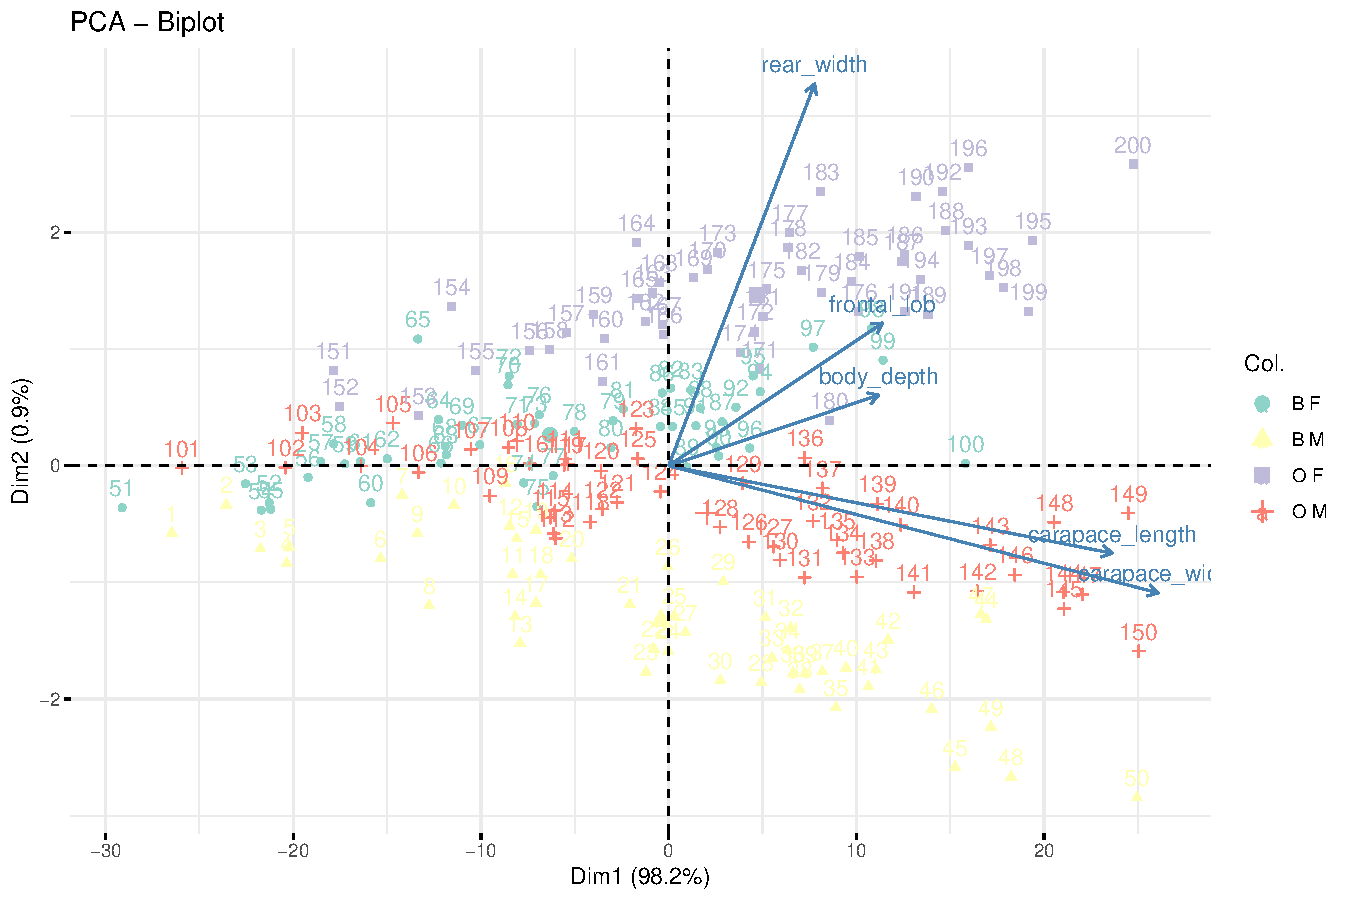
\includegraphics[width=.8\textwidth]{figures/biplot1_crabs_untransformed-1} 

\end{knitrout}
\end{frame}

\begin{frame}[fragile]
  \frametitle{Biplot (2)}
\begin{knitrout}\scriptsize
\definecolor{shadecolor}{rgb}{0.969, 0.969, 0.969}\color{fgcolor}\begin{kframe}
\begin{alltt}
\hlstd{FactoMineR}\hlopt{::}\hlkwd{PCA}\hlstd{(}\hlkwd{select}\hlstd{(crabs,} \hlopt{-}\hlstd{species,} \hlopt{-}\hlstd{sex),} \hlkwc{scale.unit} \hlstd{=} \hlnum{FALSE}\hlstd{,} \hlkwc{graph} \hlstd{=} \hlnum{FALSE}\hlstd{)} \hlopt
  \hlstd{factoextra}\hlopt{::}\hlkwd{fviz_pca_biplot}\hlstd{(}
    \hlkwc{axes} \hlstd{=} \hlkwd{c}\hlstd{(}\hlnum{2}\hlstd{,}\hlnum{3}\hlstd{),} \hlkwc{col.ind} \hlstd{=} \hlkwd{paste}\hlstd{(crabs}\hlopt{$}\hlstd{species, crabs}\hlopt{$}\hlstd{sex),} \hlkwc{palette} \hlstd{= pal}
  \hlstd{)}
\end{alltt}
\end{kframe}
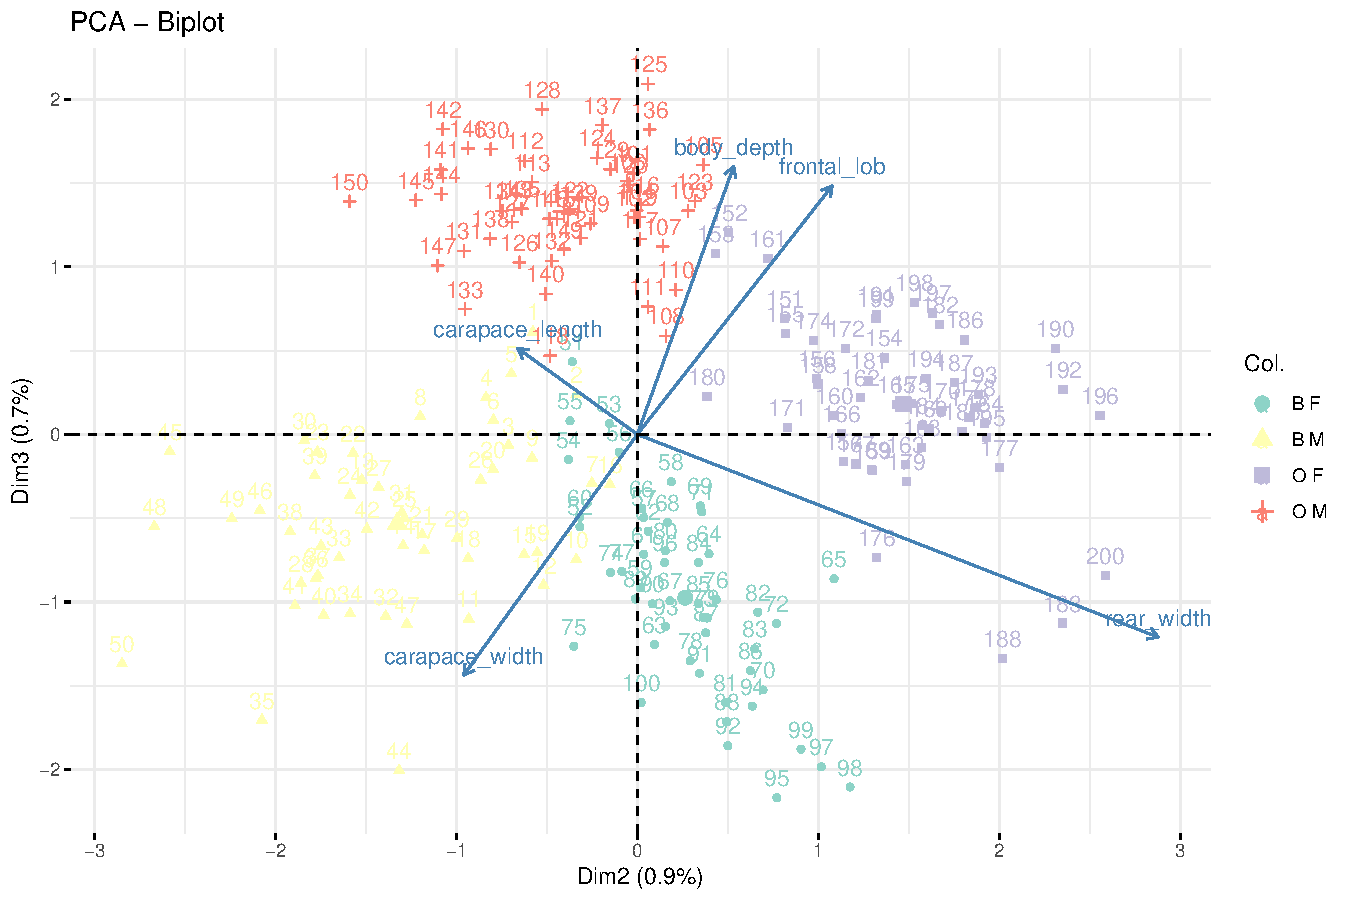
\includegraphics[width=.8\textwidth]{figures/biplot2_crabs_untransformed-1} 

\end{knitrout}
\end{frame}

\begin{frame}
  \frametitle{Reconstruction formula}

    Recall that $\mathbf{F} = (\mathbf{f}_1, \dots, \mathbf{f}_d) $ is the matrix of Principal components. Then,  
    \begin{itemize}
      \item  $\mathbf{f}_k = \bX^c \bu_k$ for projection on axis $k$
      \item $\mathbf{F} = \bX^c \bU$ for all axis.
    \end{itemize}
    Using orthogonality of $\bU$, we get back the original data as follows, without loss ($\bU^T$ performs the inverse rotation of $\bU$):
    \begin{equation*}
      \bX^c = \mathbf{F}\bU^\top 
    \end{equation*}

    \vfill
    \pause 
    
    We obtain an approximation $\tilde\bX^c$ (compression) of the data $\bX^c$ by considering a subset $\mathcal{S}$ of PC, typically $\mathcal{S} = {1, \dots,K}$ with $K \ll d$.
    \begin{equation*}
      \tilde\bX^c = \mathbf{F}_{\mathcal{S}}\bU_{\mathcal{S}}^\top = \bX^c \bU_{\mathcal{S}} \bU_{\mathcal{S}}^\top
    \end{equation*}
    $\rightsquigarrow$ This is a rank $K$ approximation of $\bX$ of the data the information capture by the first $K$ axes.

\end{frame}

\begin{frame}[fragile,allowframebreaks]
  \frametitle{Remove size effect}
  \framesubtitle{Carried by the 1st principal component}

\paragraph{First component}
\begin{equation*}
  \mathbf{f}_1 = \mathbf{X}^c \mathbf{u}_1.
\end{equation*}

We extract the best rank-1 approximation of $\mathbf{X}$ to remove the \textit{size effect}, carried by the first axis, and return to the original space,
\begin{equation*}
  \tilde{\mathbf{X}}^{(1)} = \mathbf{f}_1 \mathbf{u}_1^\top.
\end{equation*}


\begin{knitrout}\scriptsize
\definecolor{shadecolor}{rgb}{0.969, 0.969, 0.969}\color{fgcolor}\begin{kframe}
\begin{alltt}
\hlstd{attributes} \hlkwb{<-} \hlkwd{select}\hlstd{(crabs,} \hlopt{-}\hlstd{sex,} \hlopt{-}\hlstd{species)} \hlopt \hlkwd{as.matrix}\hlstd{()}
\hlstd{u1} \hlkwb{<-} \hlkwd{eigen}\hlstd{(}\hlkwd{cov}\hlstd{(attributes))}\hlopt{$}\hlstd{vectors[,} \hlnum{1}\hlstd{,} \hlkwc{drop} \hlstd{=} \hlnum{FALSE}\hlstd{]}
\hlstd{attributes_rank1} \hlkwb{<-} \hlstd{attributes} \hlopt \hlstd{u1} \hlopt \hlkwd{t}\hlstd{(u1)}
\hlstd{crabs_corrected} \hlkwb{<-} \hlstd{crabs}
\hlstd{crabs_corrected[,} \hlnum{3}\hlopt{:}\hlnum{7}\hlstd{]} \hlkwb{<-} \hlstd{attributes} \hlopt{-} \hlstd{attributes_rank1}
\end{alltt}
\end{kframe}
\end{knitrout}

$\rightsquigarrow$ Axis 1 explains a latent effect, here the size in the case at hand, common to all attributes.

\begin{knitrout}\scriptsize
\definecolor{shadecolor}{rgb}{0.969, 0.969, 0.969}\color{fgcolor}\begin{kframe}
\begin{alltt}
\hlkwd{ggpairs}\hlstd{(crabs_corrected,} \hlkwc{columns} \hlstd{=} \hlnum{3}\hlopt{:}\hlnum{7}\hlstd{,} \hlkwd{aes}\hlstd{(}\hlkwc{colour} \hlstd{= species,} \hlkwc{shape} \hlstd{= sex))}
\end{alltt}
\end{kframe}
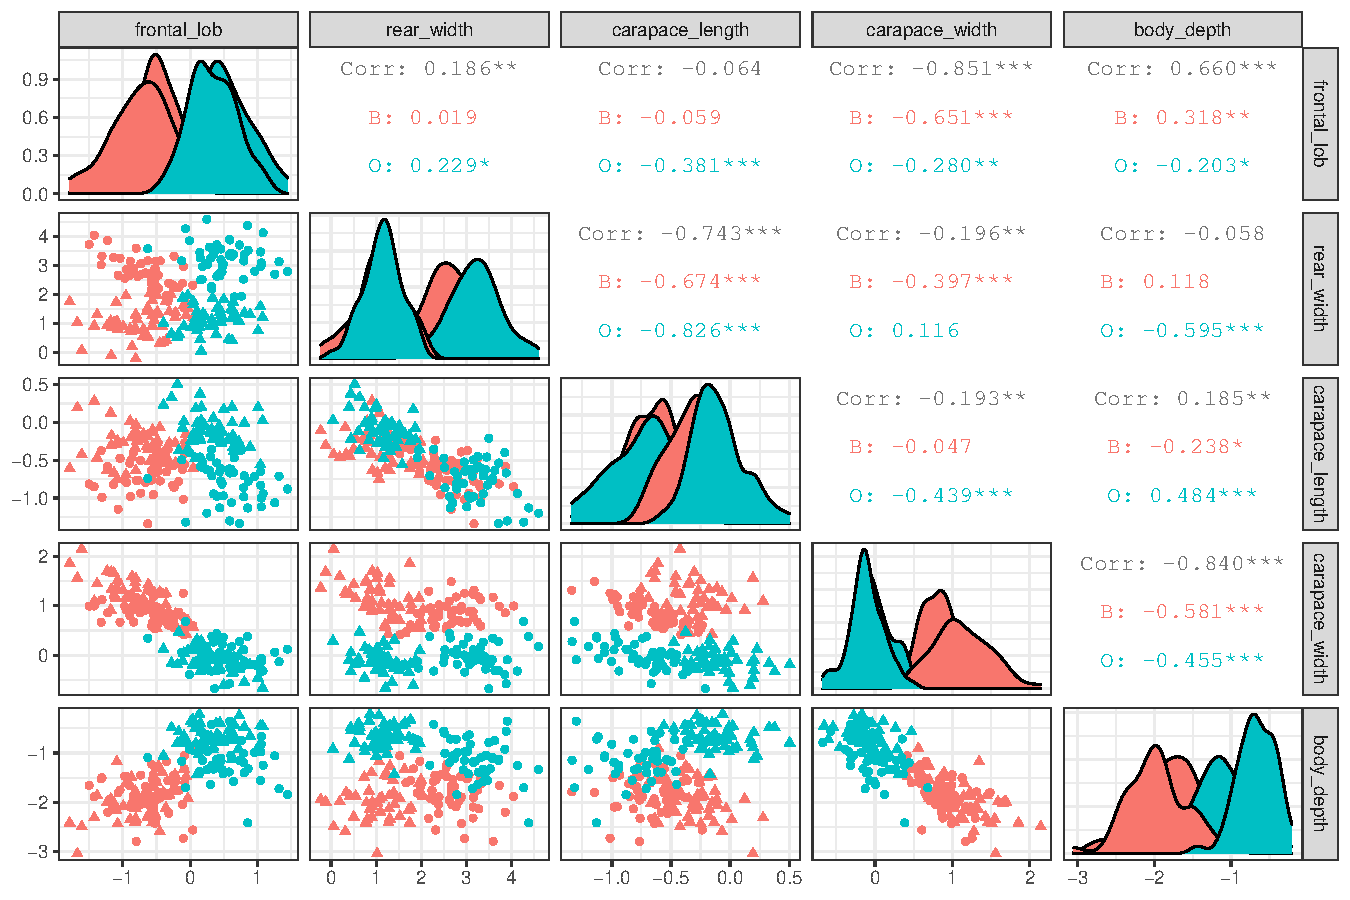
\includegraphics[width=.8\textwidth]{figures/pairs_plot_corrected-1} 

\end{knitrout}

\end{frame}

\begin{frame}[fragile]
  \frametitle{PCA on corrected data (1)}
\begin{knitrout}\scriptsize
\definecolor{shadecolor}{rgb}{0.969, 0.969, 0.969}\color{fgcolor}\begin{kframe}
\begin{alltt}
\hlstd{crabs_pca_corrected} \hlkwb{<-} \hlkwd{select}\hlstd{(crabs_corrected,} \hlopt{-}\hlstd{species,} \hlopt{-}\hlstd{sex)} \hlopt \hlstd{FactoMineR}\hlopt{::}\hlkwd{PCA}\hlstd{(}\hlkwc{graph} \hlstd{=} \hlnum{FALSE}\hlstd{)}
\hlkwd{fviz_eig}\hlstd{(crabs_pca_corrected)}
\end{alltt}
\end{kframe}
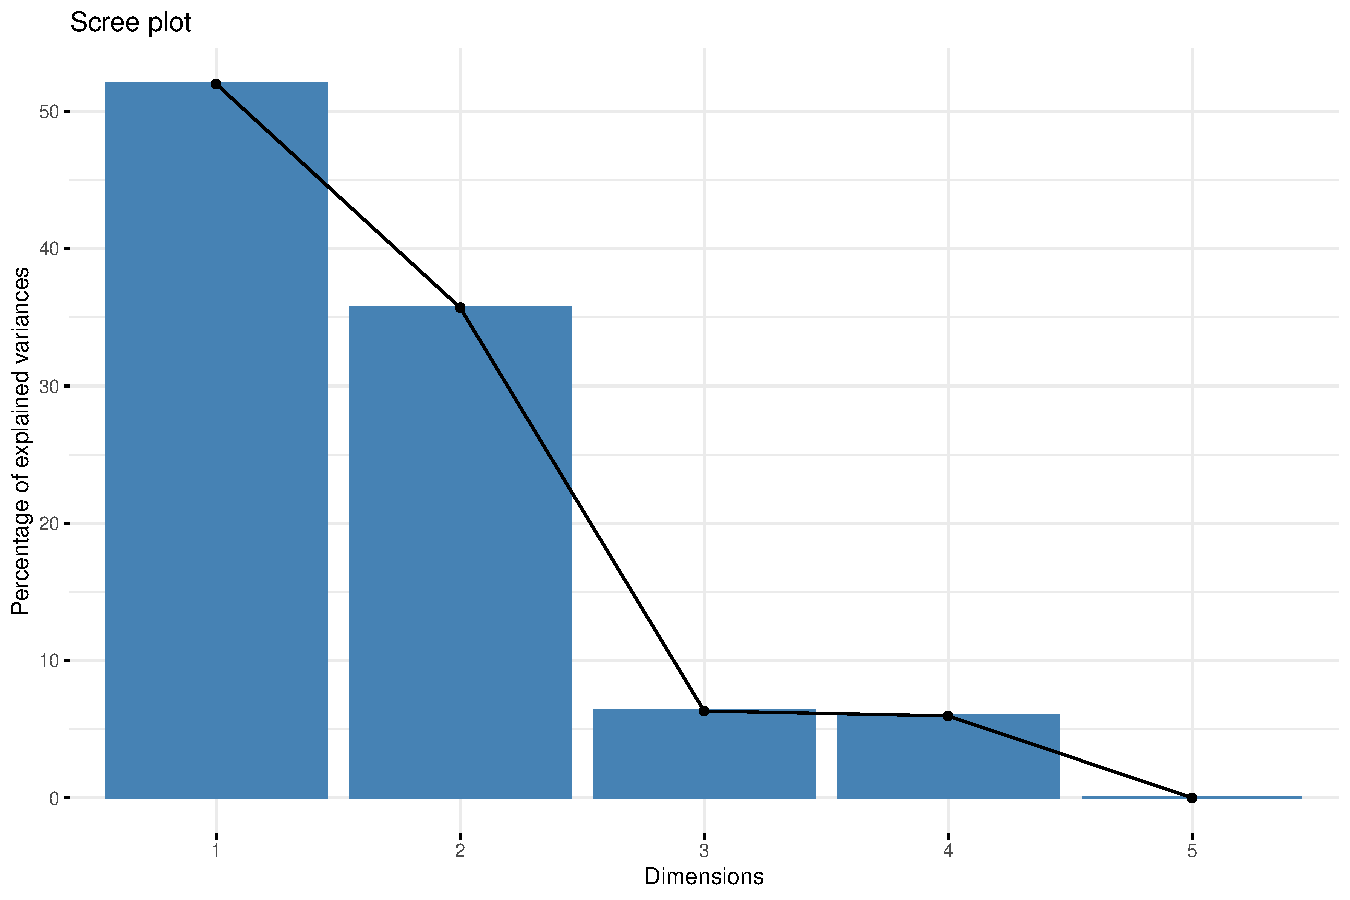
\includegraphics[width=.8\textwidth]{figures/pca_crabs_corrected_scree-1} 

\end{knitrout}
\end{frame}

\begin{frame}[fragile]
  \frametitle{PCA on corrected data (2)}
\begin{knitrout}\scriptsize
\definecolor{shadecolor}{rgb}{0.969, 0.969, 0.969}\color{fgcolor}\begin{kframe}
\begin{alltt}
\hlkwd{fviz_pca_ind}\hlstd{(crabs_pca_corrected,} \hlkwc{col.ind} \hlstd{=} \hlkwd{paste}\hlstd{(crabs_corrected}\hlopt{$}\hlstd{species, crabs_corrected}\hlopt{$}\hlstd{sex),} \hlkwc{palette} \hlstd{= pal)}
\end{alltt}
\end{kframe}
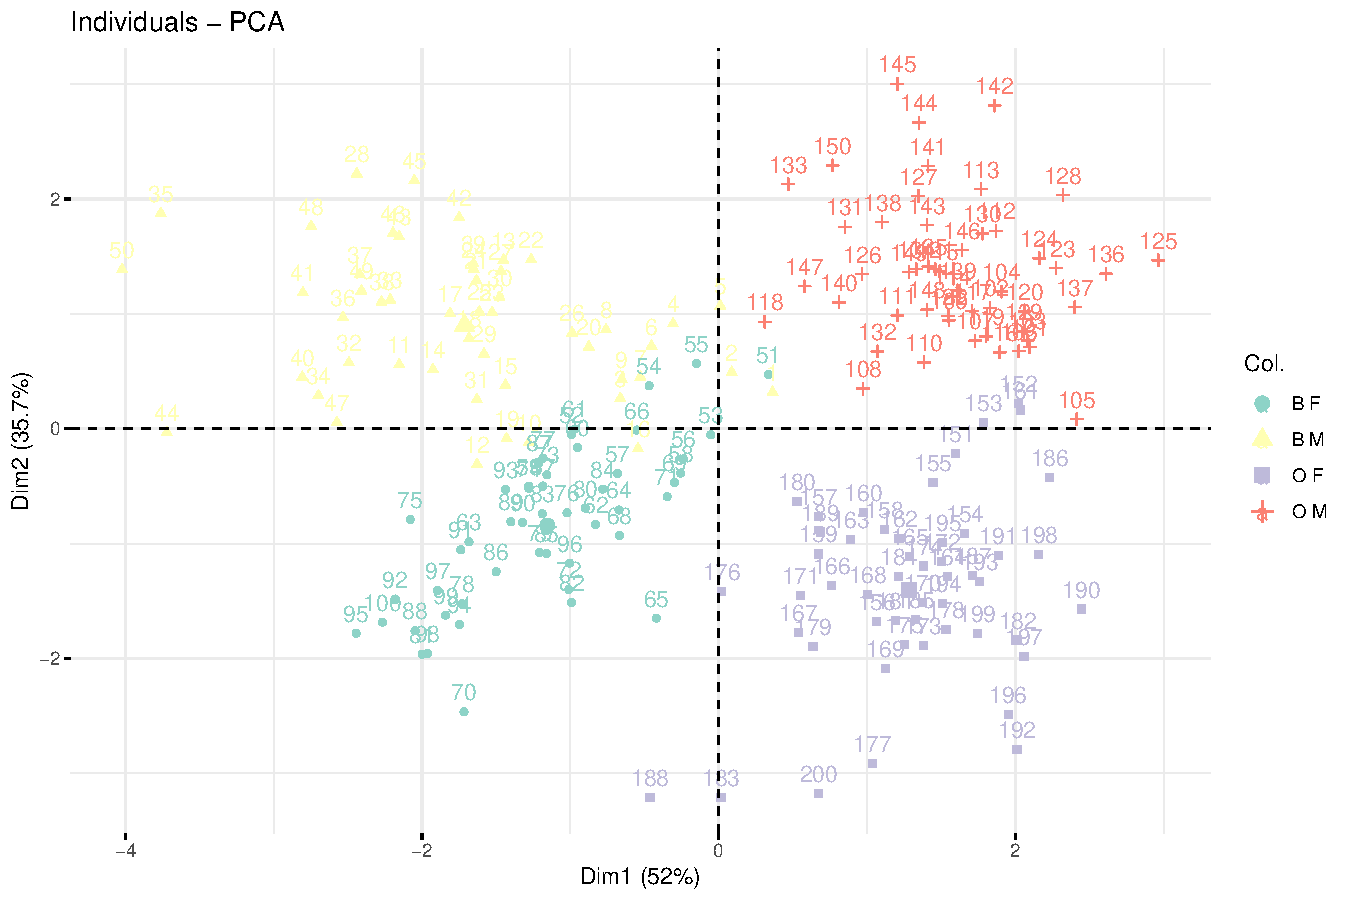
\includegraphics[width=.8\textwidth]{figures/pca_crabs_corrected_ind-1} 

\end{knitrout}
\end{frame}

\begin{frame}[fragile]
  \frametitle{PCA on corrected data (3)}
\begin{knitrout}\scriptsize
\definecolor{shadecolor}{rgb}{0.969, 0.969, 0.969}\color{fgcolor}\begin{kframe}
\begin{alltt}
\hlkwd{fviz_pca_var}\hlstd{(crabs_pca_corrected,} \hlkwc{col.var} \hlstd{=} \hlstr{'cos2'}\hlstd{)}
\end{alltt}
\end{kframe}
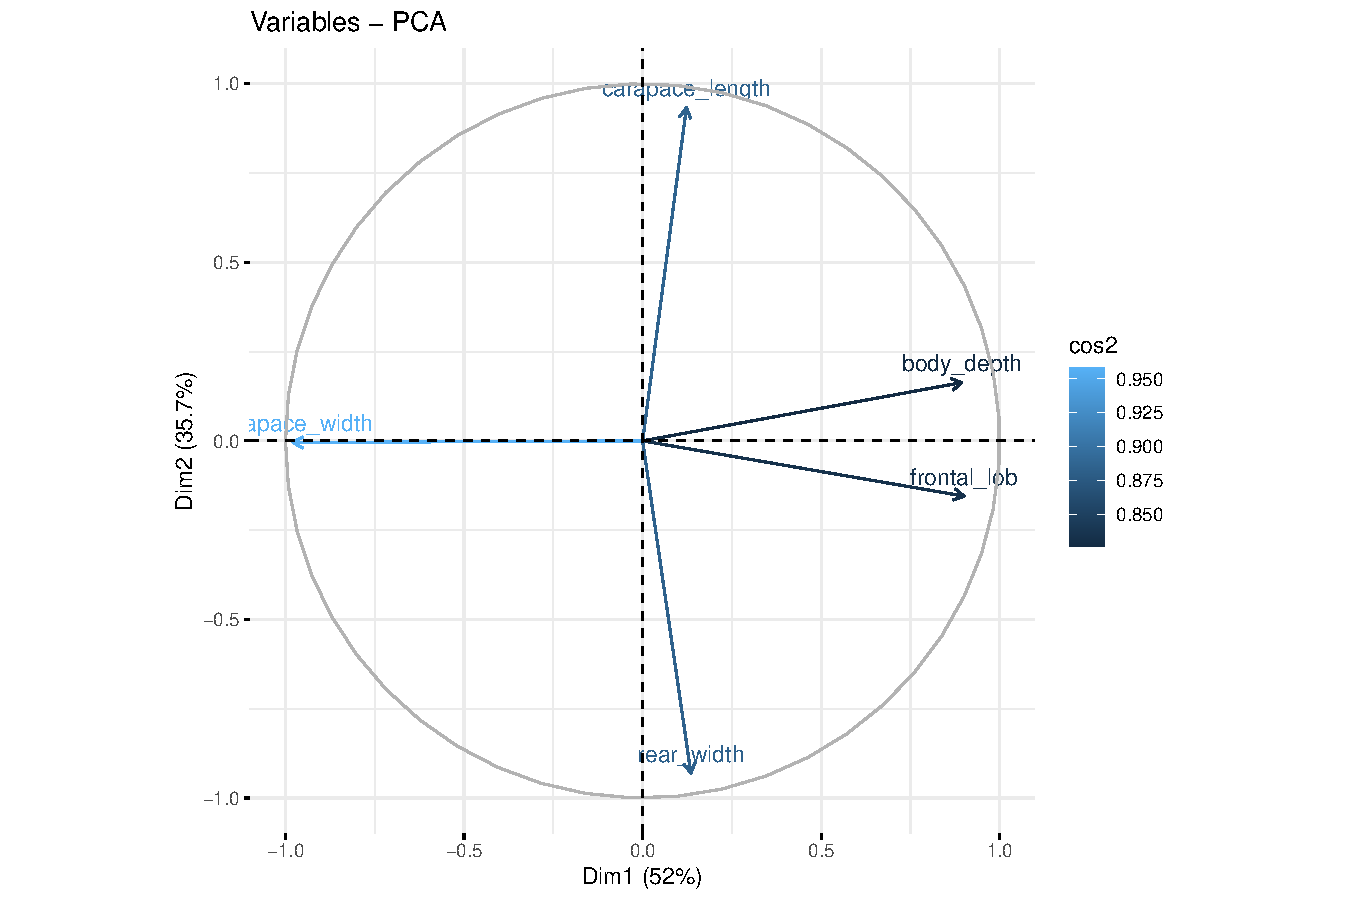
\includegraphics[width=.8\textwidth]{figures/pca_crabs_corrected_var-1} 

\end{knitrout}
\end{frame}

\begin{frame}[fragile]
  \frametitle{PCA on corrected data (3)}
\begin{knitrout}\scriptsize
\definecolor{shadecolor}{rgb}{0.969, 0.969, 0.969}\color{fgcolor}\begin{kframe}
\begin{alltt}
\hlkwd{fviz_pca_biplot}\hlstd{(crabs_pca_corrected,} \hlkwc{col.ind} \hlstd{=} \hlkwd{paste}\hlstd{(crabs_corrected}\hlopt{$}\hlstd{species, crabs_corrected}\hlopt{$}\hlstd{sex),} \hlkwc{palette} \hlstd{= pal)}
\end{alltt}
\end{kframe}
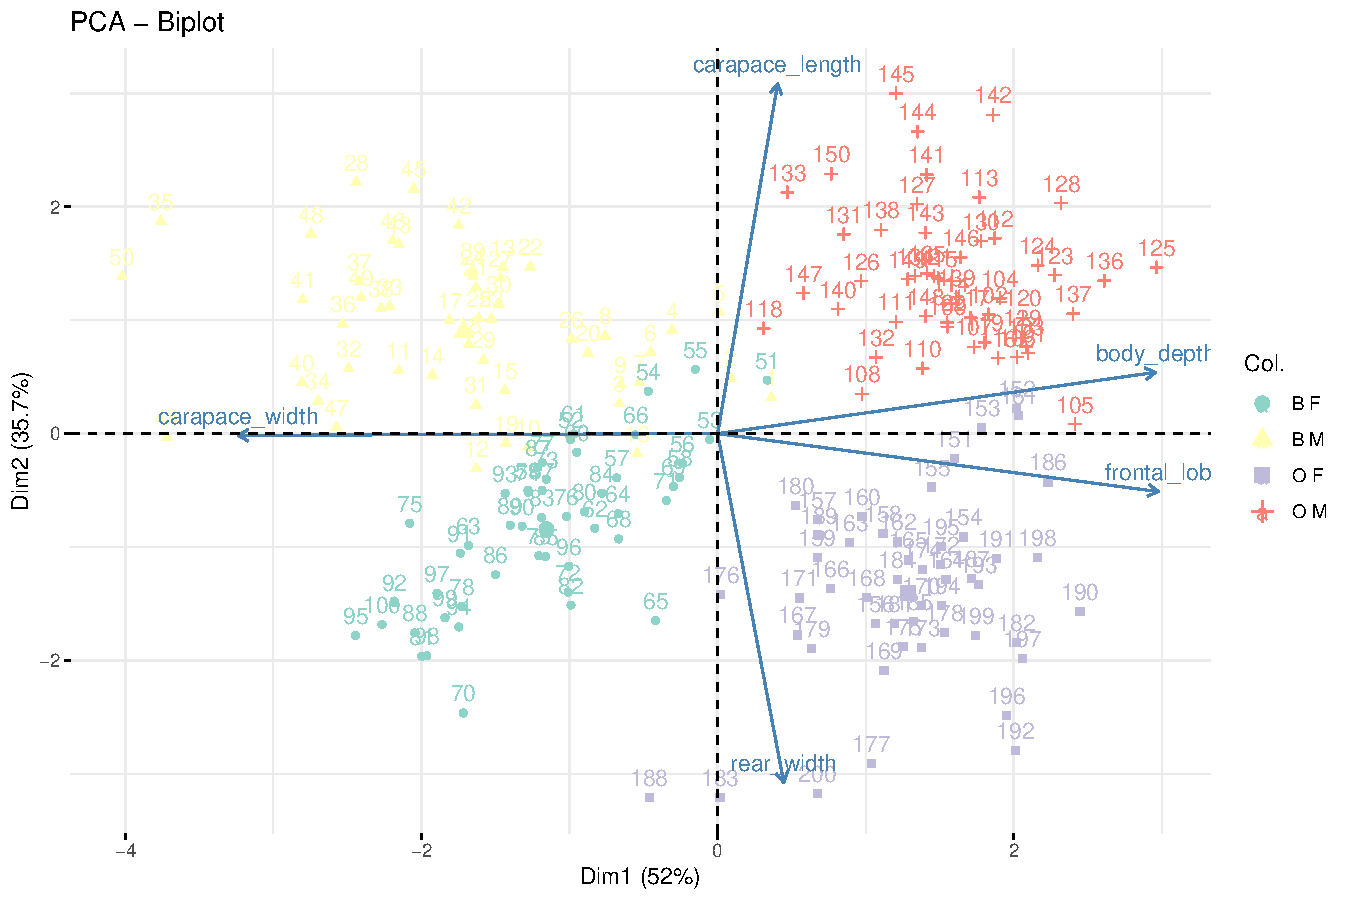
\includegraphics[width=.8\textwidth]{figures/pca_crabs_corrected_biplot-1} 

\end{knitrout}
\end{frame}

\begin{frame}
  \frametitle{Choosing the number of components}

  \begin{columns}
  \begin{column}{0.68\textwidth}
    \begin{block}{Various solutions, open question}
    Scree plot, test on eigenvalues, confidence interval, cross-validation, generalized cross-validation, etc.
    \end{block}
  \end{column}~~
  \begin{column}{0.3\textwidth}
    \includegraphics[width=\textwidth]{wine_pca_eig}
  \end{column}
  \end{columns}
  
  \begin{columns}
  \begin{column}{.5\textwidth}
  \begin{block}{Objectives}
    \begin{itemize}
      \item Interpretation
      \item Separate structure and noise
      \item Data compression    
    \end{itemize}
  \end{block}
\end{column}
\begin{column}{0.5\textwidth}
\includegraphics[width=\textwidth]{dim_reduc.pdf}
  \end{column}
  \end{columns}
\end{frame}

\begin{frame}[fragile]
  \frametitle{Example: Generalized Cross Validation}

\begin{knitrout}\scriptsize
\definecolor{shadecolor}{rgb}{0.969, 0.969, 0.969}\color{fgcolor}\begin{kframe}
\begin{alltt}
\hlstd{GCV} \hlkwb{<-} \hlkwd{select}\hlstd{(crabs_corrected,} \hlopt{-}\hlstd{species,} \hlopt{-}\hlstd{sex)} \hlopt
  \hlstd{FactoMineR}\hlopt{::}\hlkwd{estim_ncp}\hlstd{(}\hlkwc{ncp.min} \hlstd{=} \hlnum{1}\hlstd{,} \hlkwc{ncp.max} \hlstd{=} \hlnum{3}\hlstd{)}
\hlkwd{qplot}\hlstd{(}\hlnum{1}\hlopt{:}\hlkwd{length}\hlstd{(GCV}\hlopt{$}\hlstd{criterion), GCV}\hlopt{$}\hlstd{criterion,} \hlkwc{geom} \hlstd{=} \hlstr{"line"}\hlstd{)} \hlopt{+} \hlkwd{labs}\hlstd{(}\hlstr{"number of axis"}\hlstd{,} \hlstr{"GCV"}\hlstd{)}
\end{alltt}
\end{kframe}
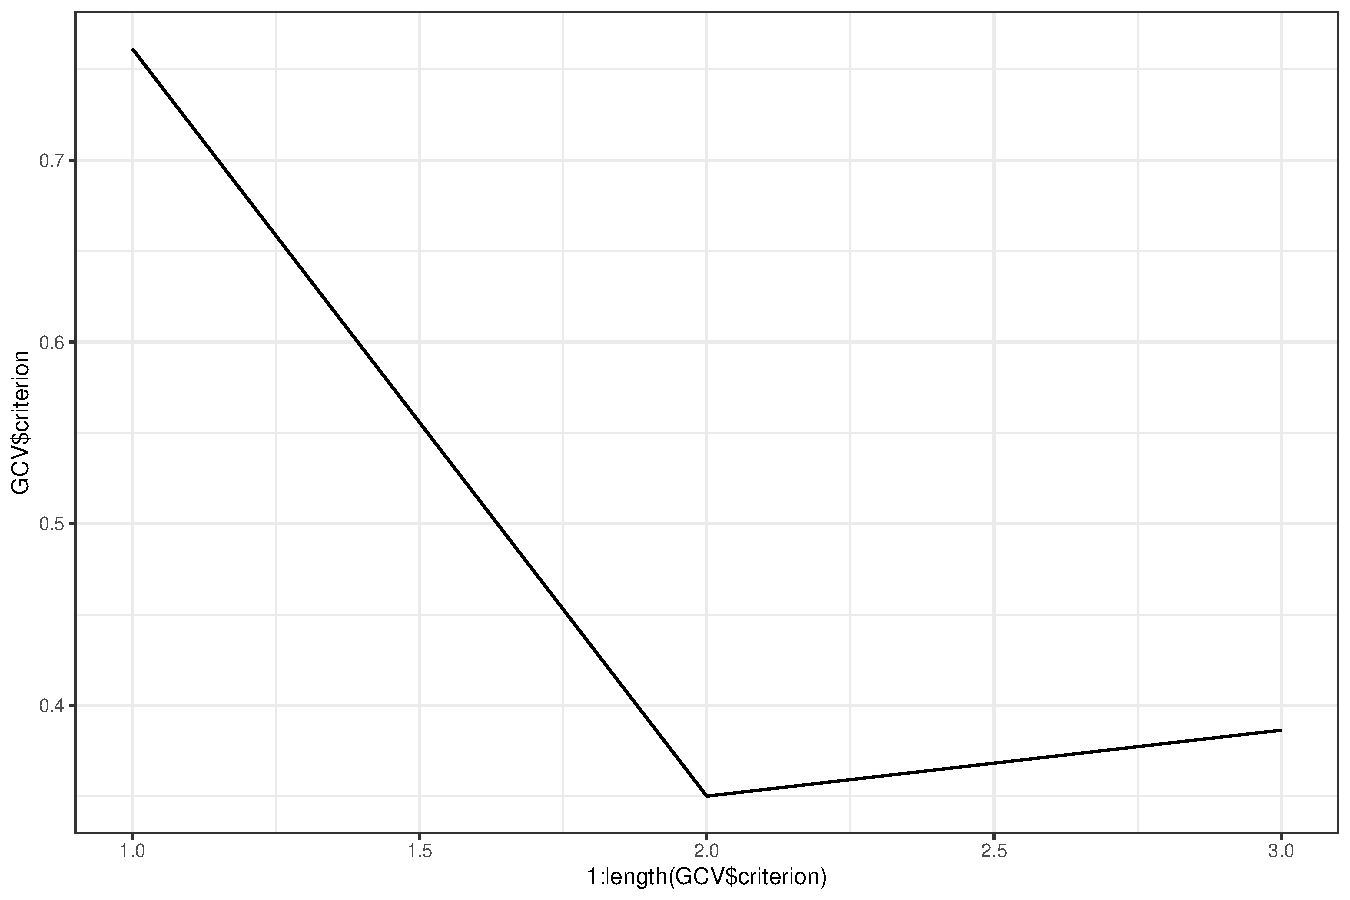
\includegraphics[width=.8\textwidth]{figures/crabs_gcv-1} 

\end{knitrout}
\end{frame}

\begin{frame}[fragile]
\frametitle{Supplementary information}
  \begin{itemize}
    \item continuous variables: projection (correlation with dimensions)
    \item observations: projection
    \item categorical variables: projection of the categories at the barycentre of the observations which take the categories
  \end{itemize}

\begin{knitrout}\scriptsize
\definecolor{shadecolor}{rgb}{0.969, 0.969, 0.969}\color{fgcolor}\begin{kframe}
\begin{alltt}
\hlstd{crabs_pca_corrected} \hlkwb{<-} \hlstd{crabs_corrected} \hlopt \hlstd{FactoMineR}\hlopt{::}\hlkwd{PCA}\hlstd{(}\hlkwc{graph} \hlstd{=} \hlnum{FALSE}\hlstd{,} \hlkwc{quanti.sup} \hlstd{=} \hlnum{7}\hlstd{,} \hlkwc{quali.sup} \hlstd{=} \hlkwd{c}\hlstd{(}\hlnum{1}\hlstd{,}\hlnum{2}\hlstd{))}
\end{alltt}
\end{kframe}
\end{knitrout}
\end{frame}

\begin{frame}[fragile]
\frametitle{Supplementary information: example (1)}
\begin{knitrout}\scriptsize
\definecolor{shadecolor}{rgb}{0.969, 0.969, 0.969}\color{fgcolor}\begin{kframe}
\begin{alltt}
\hlstd{factoextra}\hlopt{::}\hlkwd{fviz_pca_ind}\hlstd{(crabs_pca_corrected,} \hlkwc{habillage} \hlstd{=} \hlstr{"species"}\hlstd{,} \hlkwc{col.ind.sup} \hlstd{=} \hlstr{"black"}\hlstd{,} \hlkwc{addEllipses} \hlstd{=} \hlnum{TRUE}\hlstd{)}
\end{alltt}
\end{kframe}
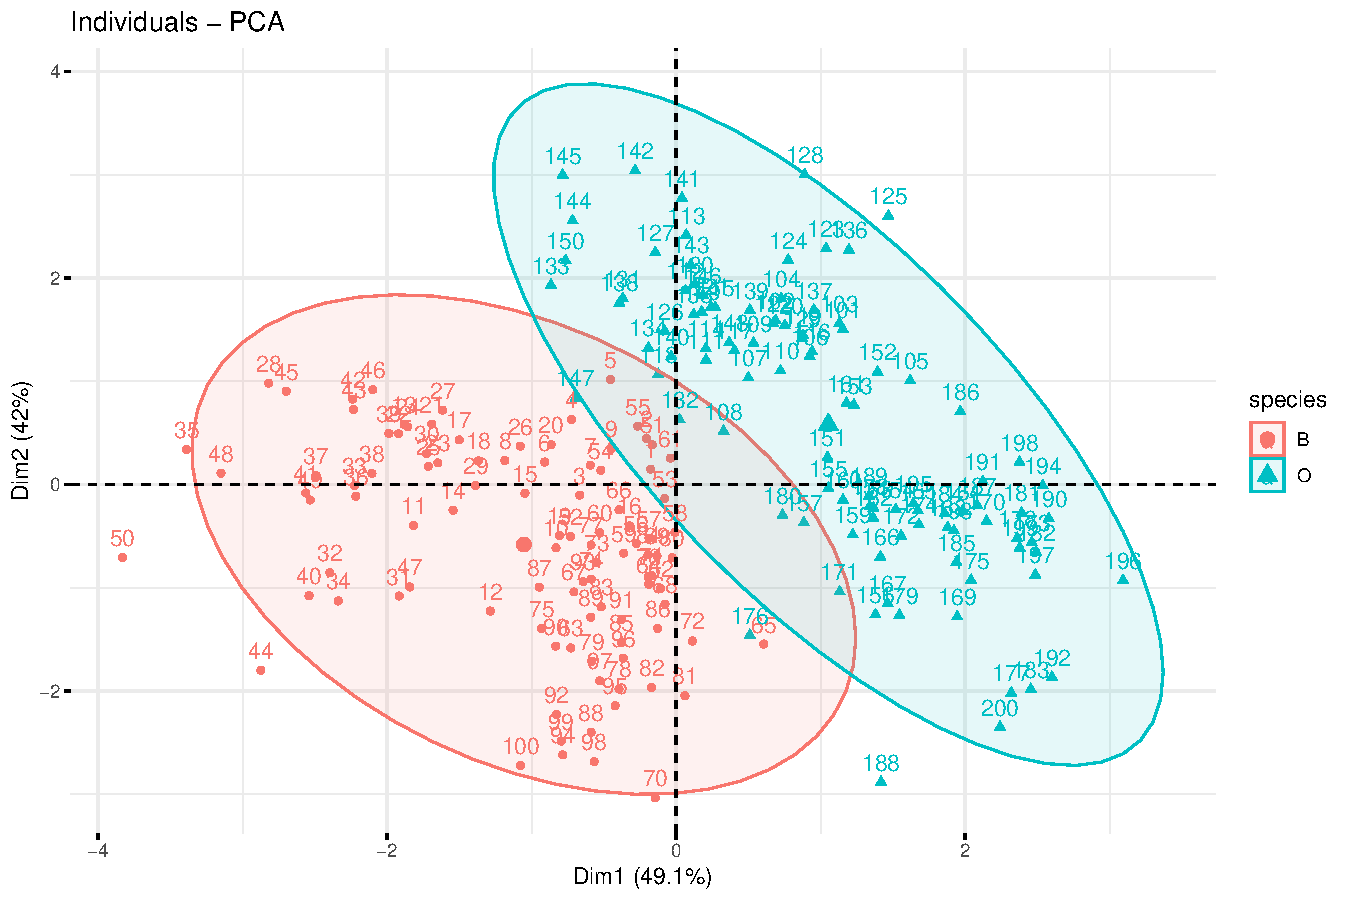
\includegraphics[width=.8\textwidth]{figures/unnamed-chunk-3-1} 

\end{knitrout}

\end{frame}

\begin{frame}[fragile]
\frametitle{Supplementary information: example (2)}
\begin{knitrout}\scriptsize
\definecolor{shadecolor}{rgb}{0.969, 0.969, 0.969}\color{fgcolor}\begin{kframe}
\begin{alltt}
\hlstd{factoextra}\hlopt{::}\hlkwd{fviz_pca_var}\hlstd{(crabs_pca_corrected)}
\end{alltt}
\end{kframe}
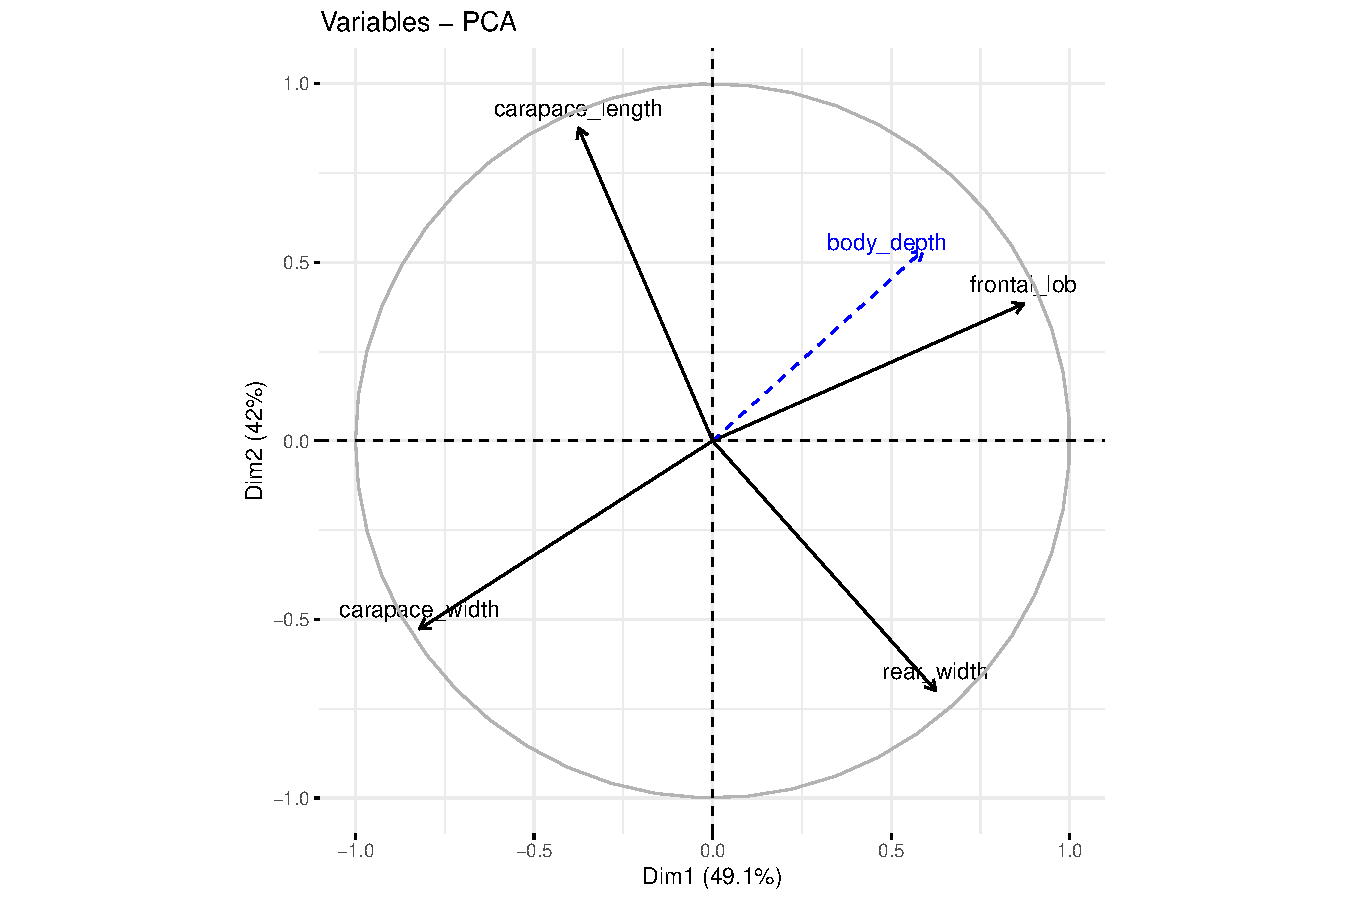
\includegraphics[width=.8\textwidth]{figures/unnamed-chunk-4-1} 

\end{knitrout}

\end{frame}

% \begin{figure}[H]
%   \includegraphics[width=0.4\textwidth]{wine_PCA_ind_mod_coul.pdf}~~\includegraphics[width=0.55\textwidth]{wine_PCA_var_supp.pdf}
% \end{figure}


\begin{frame}[fragile]
\frametitle{Description of  dimensions}
  
  \begin{block}{Using continuous variables}
    \begin{itemize}
      \item correlation between variable and the principal components
      \item sort correlation coefficients and give significant ones (rought tests)
    \end{itemize}
  \end{block}
  
  \begin{block}{Using categorical variables}
    One-way anova with the coordinates of the observations ($F_{.q}$) explained by the categorical variable
    \begin{itemize}
      \item F-test by variable
      \item for each category, a Student's $T$-test to compare the average of the category with the general mean
    \end{itemize}
  \end{block}

\end{frame}

\begin{frame}[fragile]
\frametitle{Description of  dimensions: example}
\begin{knitrout}\scriptsize
\definecolor{shadecolor}{rgb}{0.969, 0.969, 0.969}\color{fgcolor}\begin{kframe}
\begin{alltt}
\hlstd{FactoMineR}\hlopt{::}\hlkwd{dimdesc}\hlstd{(crabs_pca_corrected,} \hlkwc{axes} \hlstd{=} \hlnum{1}\hlstd{)}
\end{alltt}
\begin{verbatim}
## $Dim.1
## $quanti
##                 correlation      p.value
## frontal_lob       0.8707523 5.928707e-63
## rear_width        0.6248516 4.683973e-23
## body_depth        0.5898360 3.935692e-20
## carapace_length  -0.3755928 4.244401e-08
## carapace_width   -0.8206976 5.086379e-50
## 
## $quali
##                R2      p.value
## species 0.5653531 1.124006e-37
## sex     0.2446104 9.801298e-14
## 
## $category
##             Estimate      p.value
## species=O  1.0535355 1.124006e-37
## sex=F      0.6929897 9.801298e-14
## sex=M     -0.6929897 9.801298e-14
## species=B -1.0535355 1.124006e-37
## 
## attr(,"class")
## [1] "condes" "list " 
## 
## $call
## $call$num.var
## [1] 1
## 
## $call$proba
## [1] 0.05
## 
## $call$weights
##   [1] 1 1 1 1 1 1 1 1 1 1 1 1 1 1 1 1 1 1 1 1 1 1 1 1 1 1 1 1 1 1 1 1 1 1 1 1 1
##  [38] 1 1 1 1 1 1 1 1 1 1 1 1 1 1 1 1 1 1 1 1 1 1 1 1 1 1 1 1 1 1 1 1 1 1 1 1 1
##  [75] 1 1 1 1 1 1 1 1 1 1 1 1 1 1 1 1 1 1 1 1 1 1 1 1 1 1 1 1 1 1 1 1 1 1 1 1 1
## [112] 1 1 1 1 1 1 1 1 1 1 1 1 1 1 1 1 1 1 1 1 1 1 1 1 1 1 1 1 1 1 1 1 1 1 1 1 1
## [149] 1 1 1 1 1 1 1 1 1 1 1 1 1 1 1 1 1 1 1 1 1 1 1 1 1 1 1 1 1 1 1 1 1 1 1 1 1
## [186] 1 1 1 1 1 1 1 1 1 1 1 1 1 1 1
## 
## $call$X
##            Dim.1   species   sex  frontal_lob  rear_width carapace_length
## 1   -0.176580554 species=B sex=M  0.045978889  1.20165725    -0.605491694
## 2   -0.203793901 species=B sex=M -0.092885980  1.62897852    -0.345448656
## 3   -0.666990548 species=B sex=M -0.218411385  1.37021129    -0.535483084
## 4   -0.722489828 species=B sex=M -0.222893239  1.19407843    -0.274451365
## 5   -0.454416417 species=B sex=M -0.060818709  1.26818736    -0.153115628
## 6   -0.909810008 species=B sex=M -0.469428267  1.30655366    -0.374825783
## 7   -0.592742015 species=B sex=M -0.499086266  1.98150177    -0.258595900
## 8   -1.184595299 species=B sex=M -0.414246163  0.89807919    -0.419712369
## 9   -0.448600959 species=B sex=M -0.035370595  1.52019449    -0.348692195
## 10  -0.830614393 species=B sex=M -0.595899508  2.03753097    -0.511330209
## 11  -1.816614575 species=B sex=M -1.099126721  1.72091316    -0.284786273
## 12  -1.284704602 species=B sex=M -0.954148461  1.95161905    -0.691493253
## 13  -1.881655190 species=B sex=M -0.816325052  0.84090386    -0.127876740
## 14  -1.543364693 species=B sex=M -0.535945868  1.09577736    -0.461155822
## 15  -1.045915377 species=B sex=M -0.561334017  1.77844530    -0.313815420
## 16  -0.324003403 species=B sex=M -0.289531044  1.99573226    -0.557465081
## 17  -1.501345147 species=B sex=M -0.560820137  1.27399124    -0.135003621
## 18  -1.367635006 species=B sex=M -0.630764050  1.52624173    -0.180079906
## 19  -0.807622175 species=B sex=M -0.361339565  1.77363664    -0.536081008
## 20  -0.864764843 species=B sex=M -0.310746392  1.39856597    -0.275649810
## 21  -1.690413640 species=B sex=M -0.806255205  1.28721739    -0.033096523
## 22  -1.920485560 species=B sex=M -0.872211998  0.73738493    -0.192156883
## 23  -1.648210210 species=B sex=M -0.355207735  0.41726175    -0.449468950
## 24  -1.857634397 species=B sex=M -0.693751050  0.78614400    -0.151668815
## 25  -1.714852521 species=B sex=M -0.788516617  1.12144917    -0.248229684
## 26  -1.078230069 species=B sex=M -0.486374985  1.39117952    -0.236369526
## 27  -1.615758038 species=B sex=M -0.560188627  0.90425162    -0.104308380
## 28  -2.819967442 species=B sex=M -1.425021373  0.90904018     0.279618518
## 29  -1.386797690 species=B sex=M -0.643351968  1.40613596    -0.313894277
## 30  -1.726452239 species=B sex=M -0.398218260  0.33694797    -0.420278830
## 31  -1.916393956 species=B sex=M -1.088808185  1.06549401    -0.752686830
## 32  -2.395569082 species=B sex=M -1.382808638  1.29651663    -0.469914795
## 33  -2.225780093 species=B sex=M -0.993706135  0.89388197    -0.270264087
## 34  -2.337423983 species=B sex=M -1.133164905  1.03040756    -0.666944744
## 35  -3.386309084 species=B sex=M -1.675418985  1.02368336     0.193486486
## 36  -2.216054490 species=B sex=M -0.817176205  0.77305448    -0.341199325
## 37  -2.492772923 species=B sex=M -1.168348065  0.86504715    -0.177011096
## 38  -2.104592199 species=B sex=M -0.620109740  0.50278351    -0.354702032
## 39  -1.986799059 species=B sex=M -0.699651220  0.54848190    -0.219685402
## 40  -2.540122641 species=B sex=M -1.232912108  0.91616550    -0.633182642
## 41  -2.562422112 species=B sex=M -1.077428556  0.78097000    -0.247771862
## 42  -2.238961969 species=B sex=M -1.180565777  1.07402339     0.123466895
## 43  -2.231176873 species=B sex=M -0.892068073  0.80270756     0.014445115
## 44  -2.873441882 species=B sex=M -1.791656777  1.74242735    -0.610808246
## 45  -2.697258989 species=B sex=M -0.809750333 -0.22858334    -0.111247406
## 46  -2.098428353 species=B sex=M -0.451525060  0.31597094    -0.068223612
## 47  -1.843140447 species=B sex=M -0.808064547  1.29949434    -0.637422892
## 48  -3.149261617 species=B sex=M -1.173924105 -0.11854003    -0.303699596
## 49  -2.532096438 species=B sex=M -0.863490896  0.19338743    -0.459805157
## 50  -3.832047157 species=B sex=M -1.611941172  0.05840880    -0.423496362
## 51  -0.165058423 species=B sex=F -0.087874690  1.52469233    -0.416365904
## 52  -0.731154389 species=B sex=F -0.550943120  1.97973414    -0.510377795
## 53  -0.077980409 species=B sex=F -0.087591698  1.82778795    -0.556721443
## 54  -0.520234064 species=B sex=F -0.329266543  1.76280066    -0.357998638
## 55  -0.265493698 species=B sex=F -0.078396896  1.66099191    -0.267321876
## 56  -0.276469764 species=B sex=F -0.350730906  1.97026925    -0.654445788
## 57  -0.187134287 species=B sex=F -0.248001254  2.23559615    -0.563620051
## 58  -0.007664897 species=B sex=F -0.243749572  2.30196212    -0.569637350
## 59  -0.363201558 species=B sex=F -0.317436798  2.38338881    -0.529895969
## 60  -0.527622619 species=B sex=F -0.315690020  1.91150813    -0.555944943
## 61  -0.038730799 species=B sex=F  0.039021895  2.31712732    -0.235044541
## 62  -0.107199219 species=B sex=F -0.168885207  2.23865610    -0.781117405
## 63  -0.728208113 species=B sex=F -0.777225362  2.61854778    -0.765178636
## 64  -0.189600862 species=B sex=F -0.559008820  2.69925220    -0.619976216
## 65   0.606450624 species=B sex=F -0.240158081  3.31692615    -0.858622303
## 66  -0.394632216 species=B sex=F -0.496519915  2.27364401    -0.397780989
## 67  -0.706863076 species=B sex=F -0.896292483  2.66418952    -0.541817417
## 68  -0.076624777 species=B sex=F -0.259991145  2.33031329    -0.829431762
## 69  -0.132099212 species=B sex=F -0.519725545  2.55299704    -0.568167732
## 70  -0.144265551 species=B sex=F -0.629086085  3.16872871    -1.339509369
## 71  -0.169688800 species=B sex=F -0.571410309  2.57156639    -0.634715465
## 72   0.113327079 species=B sex=F -0.445914802  3.15724003    -0.774415162
## 73  -0.548674999 species=B sex=F -0.839534315  2.88852271    -0.390852989
## 74  -0.586248406 species=B sex=F -0.471179586  2.20345561    -0.641654932
## 75  -0.930434679 species=B sex=F -0.573762043  2.16515602    -0.761847468
## 76  -0.192623359 species=B sex=F -0.511179450  2.83961180    -0.539457915
## 77  -0.588282683 species=B sex=F -0.522806526  2.29513760    -0.478410620
## 78  -0.395174767 species=B sex=F -0.549134943  2.77235876    -0.955274585
## 79  -0.583593746 species=B sex=F -0.945560989  2.86518888    -0.792369724
## 80  -0.026979597 species=B sex=F -0.113748064  2.38690702    -0.626383983
## 81   0.061381523 species=B sex=F -0.101446246  2.95876868    -1.015703847
## 82  -0.170091901 species=B sex=F -0.733700920  3.05887091    -0.934532047
## 83  -0.517983913 species=B sex=F -1.042644362  3.24796049    -0.475336440
## 84  -0.191713958 species=B sex=F -0.475148030  2.66711226    -0.505664771
## 85  -0.377741175 species=B sex=F -0.662313578  2.73933753    -0.793879858
## 86  -0.126698188 species=B sex=F -0.502697152  3.14830494    -0.662806615
## 87  -0.946216515 species=B sex=F -1.323305105  3.01982161    -0.372313470
## 88  -0.587538595 species=B sex=F -0.888740912  3.14822287    -0.978367021
## 89  -0.590043208 species=B sex=F -0.577295210  2.39257324    -0.739790518
## 90  -0.832170829 species=B sex=F -0.971486427  2.55519733    -0.764832190
## 91  -0.375051908 species=B sex=F -0.522054112  2.89374881    -0.640046576
## 92  -0.828099854 species=B sex=F -1.137921906  3.27330638    -0.817467404
## 93  -0.643611837 species=B sex=F -0.741095492  2.67594471    -0.501795912
## 94  -0.784637122 species=B sex=F -1.310613639  3.31887609    -0.990497245
## 95  -0.422165984 species=B sex=F -0.802388383  3.59275963    -0.766018553
## 96  -0.365387055 species=B sex=F -0.547942203  2.42992911    -0.953087361
## 97  -0.529216920 species=B sex=F -1.226364014  3.86197724    -0.582510578
## 98  -0.567302708 species=B sex=F -1.426617525  4.04738953    -0.849798650
## 99  -0.795000522 species=B sex=F -1.502131767  3.72756895    -0.813846828
## 100 -1.074984459 species=B sex=F -1.071382291  2.66107328    -1.146501226
## 101  1.154036230 species=O sex=M  0.890822909  1.29573491    -0.327313168
## 102  0.688449120 species=O sex=M  0.399066704  1.50907011    -0.128902485
## 103  1.130130111 species=O sex=M  0.635898521  1.72940968    -0.174760738
## 104  0.727626822 species=O sex=M  0.432881924  1.51293566    -0.047779949
## 105  1.619538935 species=O sex=M  1.044767232  1.57970810    -0.560217812
## 106  0.923963640 species=O sex=M  0.647549538  1.30853435    -0.384118917
## 107  0.500175421 species=O sex=M  0.044086092  1.76002357    -0.250646946
## 108  0.328527128 species=O sex=M -0.036540080  1.96363999    -0.354970298
## 109  0.535681782 species=O sex=M  0.454038237  1.26201285    -0.252258484
## 110  0.722231518 species=O sex=M  0.333298442  1.87478097    -0.224948668
## 111  0.206804326 species=O sex=M -0.113568533  1.86490764    -0.074085413
## 112  0.064370452 species=O sex=M  0.136441885  0.86731719    -0.062936763
## 113  0.069806672 species=O sex=M  0.167136206  0.98827168     0.200728792
## 114  0.205317307 species=O sex=M  0.151259630  1.17743301    -0.232202088
## 115  0.271751066 species=O sex=M  0.319648078  1.12412064    -0.090352120
## 116  0.940685117 species=O sex=M  0.639203459  1.44227564    -0.327536652
## 117  0.403895407 species=O sex=M  0.048334413  1.63889943    -0.153105570
## 118 -0.123864072 species=O sex=M  0.102507816  1.40280951    -0.170412275
## 119  0.878541127 species=O sex=M  0.604542335  1.47727162    -0.236520207
## 120  0.752972749 species=O sex=M  0.442936765  1.39387308    -0.201391401
## 121  0.242163613 species=O sex=M  0.190340658  1.32143003    -0.025321263
## 122  0.673720186 species=O sex=M  0.718621845  1.07727370    -0.251824928
## 123  1.037494624 species=O sex=M  0.498916188  1.82247952     0.170211850
## 124  0.775807297 species=O sex=M  0.624713873  1.16701798    -0.005951208
## 125  1.469008311 species=O sex=M  1.075740260  1.20665771     0.022140798
## 126 -0.079568965 species=O sex=M  0.165932752  1.03940130    -0.124308203
## 127 -0.143905462 species=O sex=M  0.083221382  0.97813078     0.181879423
## 128  0.889968713 species=O sex=M  1.009390458  0.74214231     0.195503022
## 129  0.871850999 species=O sex=M  0.658919202  1.20288157    -0.331437542
## 130  0.131700661 species=O sex=M  0.385883880  0.61168013    -0.120016103
## 131 -0.368966576 species=O sex=M  0.104907593  0.75159412    -0.010229601
## 132  0.024658086 species=O sex=M  0.077016014  1.16428472    -0.475499791
## 133 -0.865911029 species=O sex=M -0.396427549  1.00453630     0.227656856
## 134 -0.191584029 species=O sex=M  0.014473323  0.84851472    -0.234896715
## 135  0.122056999 species=O sex=M  0.305251734  0.91048759    -0.146605927
## 136  1.196461947 species=O sex=M  0.805091541  1.35171970    -0.009848060
## 137  0.952708418 species=O sex=M  0.729044542  1.06326712    -0.282419298
## 138 -0.391961325 species=O sex=M -0.093639098  0.90163504     0.011186525
## 139  0.510612993 species=O sex=M  0.483793005  1.18622833    -0.135623363
## 140 -0.034552261 species=O sex=M  0.126913840  1.24259301    -0.175855085
## 141  0.040546059 species=O sex=M  0.623352169  0.40362493     0.201921313
## 142 -0.283722086 species=O sex=M  0.147016786  0.43709743     0.376825723
## 143  0.101240893 species=O sex=M  0.344639432  0.89893786     0.057058608
## 144 -0.716606147 species=O sex=M -0.276983232  0.63322521     0.330611006
## 145 -0.785056879 species=O sex=M -0.189678185  0.52455859     0.504279386
## 146  0.185540895 species=O sex=M  0.570727384  0.44367449    -0.218502386
## 147 -0.696113061 species=O sex=M -0.169433928  0.63357411    -0.375984458
## 148  0.367437873 species=O sex=M  0.463618614  1.02921169    -0.277755419
## 149  0.177055402 species=O sex=M  0.221083059  1.24922217    -0.047580126
## 150 -0.764578218 species=O sex=M  0.164114791  0.04206261     0.026839389
## 151  1.047718788 species=O sex=F  0.154173011  2.50054390    -0.473946288
## 152  1.393942952 species=O sex=F  0.761335742  1.93716548    -0.366507520
## 153  1.229967383 species=O sex=F  0.655262426  1.91379981    -0.468120997
## 154  1.519741001 species=O sex=F  0.245979759  3.06612123    -0.624465058
## 155  1.054117328 species=O sex=F  0.175455277  2.51317049    -0.592999628
## 156  1.379711345 species=O sex=F  0.438660727  2.64190513    -1.128662375
## 157  0.884018654 species=O sex=F -0.123840636  3.15789505    -0.495391605
## 158  1.339737441 species=O sex=F  0.437685247  2.73643431    -0.652939779
## 159  1.222266827 species=O sex=F  0.148721904  3.26609079    -0.581973952
## 160  1.154685880 species=O sex=F  0.183977231  2.95362241    -0.523684102
## 161  1.179143914 species=O sex=F  0.317299480  2.27637094    -0.354567752
## 162  1.364250817 species=O sex=F  0.255874662  3.02482751    -0.626482060
## 163  1.365894766 species=O sex=F  0.144440107  3.44875304    -0.457617417
## 164  1.985286416 species=O sex=F  0.395632442  3.72023776    -0.536599231
## 165  1.673420862 species=O sex=F  0.458425159  3.19483698    -0.613773842
## 166  1.414055636 species=O sex=F  0.475246855  2.93324769    -0.808554722
## 167  1.463206587 species=O sex=F  0.493267463  3.04555006    -0.971176731
## 168  1.878819382 species=O sex=F  0.645171710  3.38098420    -0.663517966
## 169  1.945392945 species=O sex=F  0.615382087  3.31930587    -1.062397150
## 170  2.148312258 species=O sex=F  0.801962264  3.37360780    -0.705068337
## 171  1.131461142 species=O sex=F  0.396573029  2.62378231    -0.975590800
## 172  1.556962714 species=O sex=F  0.472798133  2.77581989    -0.817486192
## 173  2.461275311 species=O sex=F  1.046030865  3.46715609    -0.828498168
## 174  1.680705929 species=O sex=F  0.791337669  2.52501310    -0.864195798
## 175  2.041201952 species=O sex=F  0.796889830  3.15573029    -0.982351724
## 176  0.510330581 species=O sex=F -0.629422157  3.58201144    -0.740779909
## 177  2.319260507 species=O sex=F  0.732939329  3.70726750    -1.337250673
## 178  2.360653346 species=O sex=F  0.861384565  3.52668657    -0.778250126
## 179  1.545379844 species=O sex=F  0.347163460  3.37563660    -0.944837396
## 180  0.736490950 species=O sex=F  0.322036115  2.19021430    -0.704374068
## 181  2.390922566 species=O sex=F  1.446103885  2.78932789    -0.880272903
## 182  2.491911793 species=O sex=F  1.057442879  3.08745906    -1.001261948
## 183  2.454842874 species=O sex=F  0.854112370  4.38038050    -1.130424104
## 184  1.858587097 species=O sex=F  0.579782789  3.35656379    -0.614269164
## 185  1.939797648 species=O sex=F  0.455199126  3.57151265    -0.772678141
## 186  1.967161988 species=O sex=F  0.362660479  3.49872834    -0.209128139
## 187  2.083529775 species=O sex=F  0.605503167  3.42797631    -0.620264681
## 188  1.418318488 species=O sex=F -0.067875503  4.26827218    -1.316973433
## 189  1.335420749 species=O sex=F  0.305188088  3.25468804    -0.450590321
## 190  2.578604984 species=O sex=F  0.589672467  3.88063237    -0.667936460
## 191  2.121888014 species=O sex=F  0.959865234  2.79682007    -0.714925980
## 192  2.600933091 species=O sex=F  0.587638459  3.90617062    -1.301827469
## 193  1.922588422 species=O sex=F  0.285621306  3.63172037    -0.635683517
## 194  2.537285069 species=O sex=F  1.320919541  3.13369593    -0.710542423
## 195  1.642053434 species=O sex=F -0.008786413  3.85285519    -0.398264388
## 196  3.092757993 species=O sex=F  1.083268852  4.13011439    -0.940562930
## 197  2.485900378 species=O sex=F  1.057918782  3.00800345    -1.115397625
## 198  2.376300830 species=O sex=F  1.049580564  2.96577450    -0.647528647
## 199  2.377346325 species=O sex=F  1.257023342  2.69778239    -1.061763092
## 200  2.241836709 species=O sex=F  0.248424909  4.59961969    -1.198286228
##     carapace_width body_depth
## 1      0.559396806 -0.9077224
## 2      0.438719673 -1.3313495
## 3      0.835469106 -1.5473289
## 4      0.609361604 -1.4444635
## 5      0.422526898 -1.4817001
## 6      0.697354087 -1.2647227
## 7      0.542564367 -1.5883925
## 8      0.892008262 -1.3960112
## 9      0.701564349 -1.9203848
## 10     0.918169244 -1.8707319
## 11     1.150127158 -2.1575523
## 12     1.153110033 -1.6133910
## 13     0.981788164 -1.7726217
## 14     1.265825506 -2.1937026
## 15     0.907696434 -2.1186296
## 16     0.701059006 -1.5499474
## 17     1.021988683 -2.4126757
## 18     0.961844088 -2.2813491
## 19     1.020799393 -2.1131856
## 20     0.762869578 -1.8526127
## 21     0.912499651 -2.1318548
## 22     0.974599686 -1.4911642
## 23     1.242494337 -1.8762852
## 24     1.067360668 -2.0086790
## 25     1.050384056 -1.9017232
## 26     0.784249014 -1.8014369
## 27     0.957321340 -2.0702768
## 28     1.090303441 -2.3139508
## 29     1.022102122 -2.0428472
## 30     1.225440913 -1.7985333
## 31     1.344256233 -1.1765789
## 32     1.442147100 -1.8634225
## 33     1.304080371 -2.0795714
## 34     1.655812109 -2.0146805
## 35     1.556336433 -3.0434518
## 36     1.463458621 -2.3971658
## 37     1.330449007 -2.1401422
## 38     1.427780512 -2.2982295
## 39     1.145661188 -1.8763262
## 40     1.695737902 -1.9980841
## 41     1.506928061 -2.4363425
## 42     0.912860697 -1.9339733
## 43     1.144447766 -2.3488996
## 44     1.853044893 -2.4176158
## 45     1.356424856 -1.9444631
## 46     1.276622622 -2.5927448
## 47     1.544438871 -2.3355420
## 48     1.677800092 -1.9929394
## 49     1.588572457 -1.9881451
## 50     2.140488192 -2.4957530
## 51     0.413576728 -1.0554927
## 52     0.832022528 -1.6774533
## 53     0.563957198 -1.3207020
## 54     0.610614979 -1.5579869
## 55     0.469163965 -1.6044083
## 56     0.658739740 -1.1663461
## 57     0.707066700 -1.7600331
## 58     0.558878521 -1.4522257
## 59     0.861201735 -2.2227579
## 60     0.849355401 -1.8137770
## 61     0.603586039 -2.5618754
## 62     0.869636040 -1.7623730
## 63     1.089887285 -1.9542134
## 64     0.660557590 -1.5381443
## 65     0.590602853 -1.6250853
## 66     0.574671645 -1.5749740
## 67     0.801423701 -1.6638519
## 68     0.829346999 -1.5372923
## 69     0.534655359 -1.2923087
## 70     1.310493210 -1.7887839
## 71     0.584625610 -1.2285229
## 72     0.771961936 -1.9053069
## 73     0.670725009 -1.8917765
## 74     0.956192430 -1.9264799
## 75     1.292356707 -2.3253825
## 76     0.706685271 -1.9621202
## 77     0.822140859 -1.9699031
## 78     1.174974596 -2.0903039
## 79     0.909388896 -1.4758961
## 80     0.782228229 -2.0446610
## 81     1.252471759 -2.7289497
## 82     0.875890869 -1.4479032
## 83     0.668529496 -1.7512348
## 84     0.638915858 -1.7922304
## 85     0.910378913 -1.6759961
## 86     0.875838990 -2.3192791
## 87     0.668001709 -1.5231645
## 88     1.234024723 -2.0946775
## 89     1.018153859 -1.8870727
## 90     0.986646504 -1.4722871
## 91     0.986711784 -2.4292021
## 92     1.176611979 -2.1338828
## 93     0.856230027 -2.0424482
## 94     1.123291597 -1.4998047
## 95     1.171085708 -2.7935454
## 96     0.995746469 -1.4400882
## 97     0.855537744 -2.2007373
## 98     0.994304288 -1.8846380
## 99     0.992444341 -1.6569640
## 100    1.486349987 -1.8031590
## 101   -0.195850570 -0.6600600
## 102   -0.240358593 -0.6229024
## 103   -0.342912270 -0.6812903
## 104   -0.310472129 -0.6679038
## 105   -0.228066584 -0.4471521
## 106   -0.137541960 -0.4371544
## 107   -0.177163485 -0.3260232
## 108    0.093426436 -0.7961025
## 109   -0.041261247 -0.7108025
## 110   -0.104593167 -0.9238996
## 111   -0.114630592 -0.7572000
## 112   -0.171164570 -0.2099145
## 113   -0.300886408 -0.5797777
## 114   -0.037237646 -0.3953659
## 115   -0.080654468 -0.7282197
## 116   -0.148995846 -0.6144690
## 117   -0.201858157 -0.3946051
## 118    0.306332266 -1.4341498
## 119   -0.173163686 -0.7394181
## 120   -0.259023920 -0.3908223
## 121   -0.137371620 -0.7388301
## 122   -0.014695712 -0.9146956
## 123   -0.604621300 -0.7249609
## 124   -0.361400330 -0.5923660
## 125   -0.657685240 -0.4477159
## 126    0.127514767 -0.9264653
## 127   -0.148746720 -0.8022248
## 128   -0.457138057 -0.8910628
## 129   -0.159582112 -0.4351679
## 130   -0.071612073 -0.3977942
## 131    0.156099113 -0.9718502
## 132    0.263276705 -0.4974186
## 133    0.121350584 -1.0586293
## 134    0.104232271 -0.3515594
## 135    0.012079832 -0.6624299
## 136   -0.543479718 -0.4716696
## 137   -0.275520917 -0.2427023
## 138    0.040850724 -0.6504421
## 139   -0.110821060 -0.7726001
## 140    0.172063244 -1.0229966
## 141   -0.094014501 -1.1228607
## 142   -0.329446111 -0.4814612
## 143   -0.092812227 -0.8801625
## 144   -0.160895697 -0.4814112
## 145   -0.189962244 -0.7938756
## 146    0.051073340 -0.5472825
## 147    0.469504960 -0.5685496
## 148    0.061028322 -0.7433634
## 149   -0.054937605 -0.8651451
## 150    0.285665579 -0.9192621
## 151   -0.145877964 -0.5542654
## 152   -0.258439518 -0.7454163
## 153   -0.119882420 -0.7295817
## 154   -0.185943380 -0.6296134
## 155   -0.034301591 -0.5934074
## 156    0.349761508 -0.7150018
## 157    0.061850253 -1.1672855
## 158    0.060643695 -1.1105102
## 159    0.083183264 -1.3869587
## 160    0.005981479 -1.1487109
## 161   -0.317723418 -0.4159939
## 162   -0.032131245 -0.9654041
## 163   -0.087273415 -1.3748145
## 164   -0.312139813 -1.1281850
## 165   -0.097330145 -1.1647164
## 166    0.225339269 -1.3409344
## 167    0.366599515 -1.4232412
## 168   -0.014559771 -1.5722797
## 169    0.172426248 -1.0924459
## 170   -0.116222866 -1.4019890
## 171    0.439746296 -1.1927486
## 172    0.014272396 -0.7179081
## 173   -0.073245651 -1.5550880
## 174    0.114643678 -1.0033383
## 175    0.111510203 -1.1906211
## 176    0.345805653 -1.0910246
## 177    0.278203872 -1.1479606
## 178   -0.156667504 -1.3200320
## 179    0.265964419 -1.3249125
## 180    0.379471040 -1.2477669
## 181    0.124191413 -1.8423010
## 182   -0.123615338 -0.8202692
## 183    0.381874745 -2.4180898
## 184   -0.104157124 -1.3838033
## 185   -0.089405681 -1.1061240
## 186   -0.675052180 -0.7860829
## 187   -0.276958942 -1.0440184
## 188    0.681263518 -1.7051654
## 189    0.006473864 -1.6370619
## 190   -0.571128033 -0.5559286
## 191   -0.181452213 -0.9888273
## 192   -0.091630912 -0.3506598
## 193   -0.312095199 -0.7453744
## 194   -0.128545727 -1.7234326
## 195   -0.388905490 -0.9217190
## 196   -0.317481411 -1.2476841
## 197   -0.062407635 -0.6671243
## 198   -0.339421831 -0.9716782
## 199    0.061773477 -1.0571047
## 200    0.178703243 -1.3364834
\end{verbatim}
\end{kframe}
\end{knitrout}

\end{frame}

% %% ==========================================================================
% \section{Beyond linear methods}
% %% ==========================================================================
% 
% \subsection{Reconstruction error point of view}
% 
% \begin{frame}
%   \frametitle{Reconstruction error approach}
% 
%   \begin{enumerate}
%     \item  Construct a map $\Phi$ from the space $\Rset^{d}$ into a space $\Rset^{d'}$ of \alert{smaller dimension}:
%       \begin{align*}
%       \Phi:\quad & \Rset^d \to \Rset^{d'}, d' \ll d\\
%                & \bx \mapsto \Phi(\bx)
%       \end{align*}
%     \item Construct $\widetilde{\Phi}$ from $\Rset^{d'}$ to $\Rset^d$ (\alert{reconstruction formula})
%      \item Control an error between $\bx$ and its reconstruction $\tilde{\Phi}(\Phi(\bx))$, e.g
%       \begin{equation*}
%         \sum_{i=1}^n \left\| \bx_i - \tilde{\Phi}(\Phi(\bx_i)) \right\|^2
%       \end{equation*}
%   \end{enumerate}
% 
% \end{frame}
% 
% 
% \begin{frame}
% \frametitle{Reconstruction error and PCA}
% 
%   \begin{block}{PCA Model}
%     Linear model assumption
%     \begin{equation*}
%         \bx \simeq \bmu + \mathbf{F}_{1:d'} \bU_{1:d'}^\top
%       \end{equation*}
%       with $\bU$ orthonormal and no  constraint on $\mathbf{F}$
%     \end{block}
%     
%   \begin{block}{Reconstruction error}
%     In the case of PCA, then
%     \begin{gather*}
%       \Phi(\bx) = (\bx-\bmu)^\top \bU  \quad \text{and} \quad \tilde{\Phi}(\mathbf{F})= \bmu + \mathbf{F} \bU^\top  \\
%       \frac{1}{n} \sum_{i=1}^n \| \bx_i  - ( \bmu + ( \bx_i -\bmu) \bU \bU^\top \|^2
%     \end{gather*}
%   \alert{Explicit solution:} $\bmu = \bar{x}$ the empirical mean
%  and $\bU$ is an orthonormal basis of the space spanned by the $d'$
%  first eigenvectors of the empirical covariance matrix
%   \end{block}
% \end{frame}
% 
% \begin{frame}
%   \frametitle{Non linear extensions}
% 
%   Two directions
%   \begin{enumerate}
%     \item Non linear transformation of $\bx$ before PCA: kernel-PCA
%     \item Other constrains on weigths $\bU$ or loadings $\mathbf{F}$: ICA, NMF, \dots
%   \end{enumerate}
% 
%   \begin{block}{Kernel PCA}
%     Linear assumption after transformation, with $\bU$ orthonormal and no  constraint on $\mathbf{F}$
%     \begin{equation*}
%         \Psi(\bx - \bmu) \simeq  \mathbf{F}_{1:d'} \bU_{1:d'}^\top
%       \end{equation*}
%    \end{block}
% 
%   \vfill
% 
%   \begin{block}{Non negative Matrix factorisation}
%     Linear model assumption  with $\bU$ non-negative and  $\mathbf{F}$ non-negative
%     \begin{equation*}
%         \bx \simeq \bmu + \mathbf{F}_{1:d'} \bU_{1:d'}^\top
%       \end{equation*}
%   \end{block}
%   
%   \vfill
% 
%   \paragraph{Auto-encoders} Find $\Phi$ and $\tilde\Phi$ with a neural-network!
% 
%   $\rightsquigarrow$ Fit $\bU, \mathbf{F}$ with some optimization algorithms (much more complex!)
% \end{frame}
% 
% 
% \subsection{Relation preservation point of view}
% 
% \begin{frame}
%     \frametitle{Pairwise Relation}
%   
%     Focus on pairwise relation $\mathcal{R}(\bx_i, \bx_{i'})$.
% 
%     \begin{block}{Distance Preservation}
%       \begin{itemize}
%     \item  Construct a map $\Phi$ from the space $\Rset^{d}$ into a space $\Rset^{d'}$ of \alert{smaller dimension}:
%       \begin{align*}
%       \Phi:\quad & \Rset^d \to \Rset^{d'}, d' \ll d\\
%                & \bx \mapsto \Phi(\bx)
%       \end{align*}
%       \begin{equation*}
%       \text{such that} \quad \mathcal{R}(\bx_i, \bx_{i'}) \sim\mathcal{R'}(\bx'_i, \bx'_{i'})
%       \end{equation*}
%     \end{itemize}
%   \end{block}
% 
%   \begin{block}{Multidimensional scaling}
%     Try to preserve inner product related to the distance (e.g. Euclidean)
%   \end{block}
% 
%   \vfill
%   
%   \begin{block}{t-SNE -- Stochastic Neighborhood Embedding}
%     Try to preserve relations with close neighbors with Gaussian kernel
%   \end{block}
% 
% \end{frame}



\end{document}
